% 分析型论文正文初稿 v0（2026-10-05）
% 版式：通用 article 双栏，投稿前替换为目标会议模板（CVPR/ICCV/NeurIPS 等）。
% 约定：\src{...} 标出每个数字的出处（结果文件），终稿把 \showsrcfalse 打开即隐藏。
%       \PH{...} 为占位，注明原因；不得在占位处填未核对的数字。
\documentclass[10pt,twocolumn]{article}
\usepackage[margin=0.8in]{geometry}
\usepackage{amsmath,amssymb,amsthm}
\usepackage{booktabs,multirow}
\usepackage{graphicx}
\usepackage{adjustbox}
\usepackage[T1]{fontenc}
\usepackage{lmodern}
\usepackage{microtype}
\setlength{\emergencystretch}{2em}
\usepackage[dvipsnames]{xcolor}
\usepackage[colorlinks=true,citecolor=blue,linkcolor=blue]{hyperref}
\usepackage{natbib}

\newif\ifshowsrc \showsrcfalse
\newcommand{\src}[1]{\ifshowsrc{\textcolor{gray}{\scriptsize[src: #1]}}\fi}
\newcommand{\PH}[1]{\par\noindent\fcolorbox{red}{yellow!20}{\parbox{\dimexpr\linewidth-2\fboxsep-2\fboxrule\relax}{\footnotesize\textbf{PLACEHOLDER:} #1}}}
\newcommand{\TODO}[1]{\textcolor{red}{\footnotesize[TODO: #1]}}

\newtheorem{proposition}{Proposition}
\newtheorem{corollary}{Corollary}
\theoremstyle{definition}\newtheorem{definition}{Definition}

\newcommand{\Rlin}{R_b^{\mathrm{lin}}}
\newcommand{\Rnet}{R_b^{\mathrm{net}}}

\title{Frequency Recovery and Readout Effects\\
in Arbitrary-Scale Super-Resolution}
\author{Working research draft}
\date{Revised 11 October 2026}

\begin{document}
\maketitle

\begin{abstract}
Arbitrary-scale super-resolution (ASISR) predicts pixels at continuous coordinates, but recovery above the low-resolution Nyquist frequency and the role of scale-dependent readout remain difficult to assess. We study frequency recovery and signed paired readout losses, separating input sampling, target measurement and network cell conditioning. Across three datasets, normalising frequency by the sampling scale reduces variation in all nine evaluated model--dataset groups; the pre-specified collapse tolerance nevertheless passes only six. Evaluated decoders exhibit similar recovery in 10 of 12 low-reference-recovery cells, without establishing a universal decoder limit. Two further training seeds support coarse readout-loss ordering in all four architecture--seed groups. The three-valued footprint predictor has the same Spearman ranks as band index, so this result does not validate its quantitative form. Averaging a full model over training-scale cell inputs predicts loss ordering, but fails function similarity in all four groups and improves on the footprint score in only two. Additional frozen-weight probes improve integral-forecast magnitude for SC-INR but miss negative benefits; neither tested forecast meets the complete criterion. Negative readout benefits and these failed stronger tests delimit what the baseline establishes: empirical scale and frequency structure, rather than a shared integral-readout mechanism or an adaptive model-selection rule.
\end{abstract}

\section{Introduction}\label{sec:intro}
Arbitrary-scale super-resolution (ASISR) reconstructs a high-resolution image from a low-resolution image and predicts its value at arbitrary coordinates. Local implicit decoders such as LIIF and LTE combine learned image features with coordinates and a target pixel size \citep{chen2021liif,lee2022lte}. When input sampling and target resolution vary together, their effects on observable frequencies, desired pixel measurements and network conditioning can be confounded. Aggregate PSNR can obscure which frequency bands improve, and a successful readout ablation does not explain why it improves them.

This paper asks two linked empirical questions: \emph{how does recovery change with frequency relative to the sampling scale, and where does a scale-dependent readout affect that recovery?} We make ASISR frequency recovery and paired readout behaviour the central objects of analysis. Spectral adaptation---changing a representation's preferred frequencies through Fourier features, activation scales or a covariance prior---provides context \citep{tancik2020fourier,sitzmann2020siren,kania2025fresh}. We do not propose another decoder or claim a general rule for selecting one.

Our measurement is the fraction of band energy recovered, relative to zero reconstruction of the centred signal. We compare trained networks with two specified stationary linear estimators and study frequency in low-resolution Nyquist units, $u=2s\nu$. A covariance-conditioned Wiener reference distinguishes an assumed prior from the empirical recovery of a trained network. It does not bound all possible estimators on a natural image. The stationary references are conditional comparisons; their classical formulas and auxiliary guidance tests are supplementary, rather than independent contributions to ASISR mechanism.

The strongest positive result concerns coarse structure. Frequency normalisation improves scale consistency in nine of nine model--dataset groups. Readout losses generally increase across three frequency bands, and this ordering replicates in two additional training seeds for two architecture pairs. However, the three increasing footprint scores have the same Spearman ranks as band index, so their formula is not validated by that correlation. The stronger accounts fail. Normalisation does not meet the original collapse tolerance in three groups. A predictor based on linear recovery fails the original readout-loss correlation threshold. Scale marginalisation does not reproduce the ablated function, and its advantage over the simpler footprint predictor is architecture-dependent. We preserve these failures rather than replacing the hypotheses after seeing results.

\paragraph{Contributions and scope.}
\begin{enumerate}
\item An ASISR frequency-recovery baseline that separates covariance-conditioned linear references from measured network recovery, and records scale dependence across Set14, BSD100 and Urban100.
\item A replicated paired readout analysis, extended by frozen-weight target/hint probes: coarse ordering is supported in four architecture--seed groups, whereas quantitative prediction, function-equivalence and shared mechanism claims are evaluated with their counterexamples.
\end{enumerate}
Prior work already studies cell-size interventions, integrated positional encoding and analytic anti-aliasing \citep{chen2021liif,liu2021ipe,becker2025thera}. We do not claim to introduce those principles. The linear-reference formulas are classical tools \citep{kay1993estimation,rasmussen2006gp}; the contribution claimed here is the organised empirical evidence and its scope. We distinguish original observations, pre-specified tests, independent reimplementations, saved-record audits and exploratory development. Extended protocols and results accompany the main text in the supplement.

\section{Related Work}\label{sec:related}

\paragraph{ASISR and scale-dependent readout.}
LIIF \citep{chen2021liif} conditions local decoding on a two-dimensional
cell. Its original ablation already varies cell size at fixed $\times30$
queries and discusses area averaging. LTE \citep{lee2022lte} estimates
local Fourier amplitude and frequency, with cell size entering a learned
phase estimator. The examined SC-INR implementation modulates features
with sinc factors and includes separate scale-consistency components.
These constructions are distinct; common band ordering does not prove a
shared integration mechanism. MetaSR \citep{hu2019metasr}, SRNO
\citep{wei2023srno}, CiaoSR \citep{cao2023ciaosr} and HIIF
\citep{jiang2025hiif} further develop continuous decoders, while a
controlled re-training benchmark \citep{nasir2026empirical} examines
architecture and recipe effects.

\paragraph{Integrated encoding and analytic filtering.}
IPE-LIIF \citep{liu2021ipe} integrates sinusoidal positional encodings over
a pixel area, yielding sinc attenuation, and compares this encoding with
plain positional encoding and an additional cell input. Thus neither
area-dependent encoding nor its comparison with learned cell conditioning
is new here. Thera \citep{becker2025thera} uses neural heat fields with
analytic Gaussian filtering for arbitrary-scale readout; Gaussian-splatting
decoders \citep{chen2025gsasr} offer another representation. Integrating
features before a nonlinear RGB decoder is different from a certified
integral of its output, and box and Gaussian target measurements must be
distinguished. Our current evidence measures paired frequency recovery;
it does not establish an advantage over these integral-readout methods.

\paragraph{Frequency diagnostics.}
HyRA \citep{fsds2024} studies impulse responses and a linear/nonlinear
response decomposition, and introduces Frequency Spectrum Distribution
Similarity (FSDS); it is not limited to one global scalar. Our measurement
instead compares signal-normalised reconstruction error in stated bands
and LR Nyquist units. Fourier ring correlation
\citep{vanheel2005frc} and scale-decomposed skill scores are related
agreement diagnostics. We claim neither the first frequency analysis of
SR nor a new information measure.

\paragraph{Spectral control and inverse-problem references.}
SIREN \citep{sitzmann2020siren}, Fourier features
\citep{tancik2020fourier,jacot2018ntk} and FINER \citep{liu2024finer}
control a representation's frequency preference. FreSh
\citep{kania2025fresh}, WINNER \citep{winner2025}, SEC \citep{sec2026}
and WIEN-INR \citep{wieninr} use spectral summaries or multiresolution
components. These signal-fitting and inverse-task studies differ from
our primary pretrained ASISR setting. SuperF \citep{superf2026}, DIP
\citep{ulyanov2018dip} and GP regression \citep{rasmussen2006gp} provide
context for the supplementary inverse checks. Classical LMMSE and
sampling analysis \citep{kay1993estimation} supply conditional linear
references, not a natural-image recovery ceiling. Spectral bias
\citep{rahaman2019spectral} also does not identify a trained decoder's
scale-readout mechanism.

\paragraph{Risk estimates and observation consistency.}
Generalized SURE \citep{eldar2008gsure} supplies risk-based regularization selection under its declared distributional assumptions. A bicubic-reference error difference is instead a prior-dependent proxy, with no unbiased-risk guarantee here. Range/null-space SR \citep{wang2023nullspace} already distinguishes measurement-consistent reconstruction from prior-dependent unobserved components. We do not claim this distinction or a quadratic error identity as a new principle; whether such a proxy forecasts harmful cell intervention beyond simple controls requires a separate held-out comparison.

\section{ASISR Setting and Recovery Measurement}\label{sec:setup}

\paragraph{Three distinct objects.} Let $x$ denote a continuous signal and
$y=Ax+n$ its low-resolution observation. The input operator $A$ specifies
blur, sampling and any observation noise. The desired target at coordinate
$q$ is $(Q_hx)(q)$, where $Q_h$ is a stated output measurement, such as a
point value or an average over a pixel with shape $h$. The cell input $c$
is a network conditioning variable. A protocol may set $c=h$, but this
assignment does not prove that the network computes $Q_h$. Changing $A$,
$Q_h$ and $c$ are different interventions.

\paragraph{Pretrained ASISR, not per-image fitting.} Our primary ASISR
models are amortised predictors $\hat x(q)=F_\theta(y,q,c)$: their encoder
and decoder are trained across images, then held fixed during inference.
The supplementary inverse tasks instead fit a representation $f_\theta$
to an individual observation, for example by minimising
$\|Af_\theta-y\|^2$ with stated regularisation. Their optimisation and
linear references do not identify the mechanism of a pretrained decoder.
The historical natural-image targets are discrete HR arrays with
bicubic LR preparation; they are not certified box integrals of a known
continuous field. We therefore use pixel-footprint terminology to describe
the supplied cell and implemented modulation, without assuming a matched
physical output operator for those targets.

\paragraph{Empirical recovery.} For a stated crop, colour conversion and
window, let $\Pi_b$ project onto frequency band $b$. For a reconstructed
image $\hat x$, the empirical score is
$R_b=1-\|\Pi_b(x-\hat x)\|^2/\|\Pi_b(x-\bar x)\|^2$;
for a network we write $\Rnet$. It measures error relative to a centred
zero reconstruction, uses HR truth, and may be negative. Write $S_{ib}$
and $E_{ib}$ for the signal and error energy in image $i$. The pooled
measurement is
\begin{equation}\label{eq:pooled}
R_b^{\rm emp}=1-\frac{\sum_i E_{ib}}{\sum_i S_{ib}}.
\end{equation}
It is not an unweighted mean of per-image recoveries.

\paragraph{Conditional linear reference.} For a specified centred signal
law $P$, input operator $A$ and noise covariance, the LMMSE estimator
minimises expected squared error among linear estimators. We denote its
band recovery by
\[
\Rlin=1-\frac{\mathbb E\|\Pi_b(x-\hat x_{\rm LMMSE}(P))\|^2}
{\mathbb E\|\Pi_bx\|^2}.
\]
The generic $1/f^2$ spectrum, its amplitude and centring are assumptions;
an image-periodogram reference additionally uses target truth. Neither
is a distribution-free limit on natural-image reconstruction. Classical
GP, matrix-risk and aliasing formulas are given in
Appendix~\ref{app:linear}; scalar mismatch calculations are in
Appendix~\ref{app:mismatch}. Their solver and sampling costs are recorded
separately from the network measurements.

\paragraph{Bands and scale normalisation.} Historical image bands are
square annuli in HR pixel units, indexed by $\max(|\nu_x|,|\nu_y|)$:
$b_1=[0,\tfrac18)$, $b_2=[\tfrac18,\tfrac14)$,
$b_3=[\tfrac14,\tfrac12]$ cycles/pixel. At $\times4$, the upper two bands
lie above the LR Nyquist limit. L1 uses the Chebyshev radius
$\nu=\max(|k_x|,|k_y|)/240$. Seven bins in $u=2s\nu$ place the LR Nyquist
frequency at $u=1$. For each bin we take the range across
$s\in\{2,3,4\}$, then the median across bins:
\begin{equation}\label{eq:collapse}
D_{\rm in}=\operatorname{median}_{b}\left[\max_s R_b(s)-\min_s R_b(s)\right].
\end{equation}
The absolute-frequency control fixes bins at the $s=3$ reference,
$\nu=u/6$. Smaller $D_{\rm in}$ means greater consistency in this
measurement, not equality of reconstructed functions. F1/G1 use HR256
and 73 images; L1/L2 use HR240 and 74, with their own pooling conventions.

\section{Interpreting Readout Comparisons}\label{sec:zones}
LTE conditions a learned phase on cell size \citep{lee2022lte}; the
examined SC implementation instead modulates learned Fourier features
with sinc factors. These paths need not realise the same output integral.
Even analytic integration of an intermediate feature does not certify
integration of the final RGB output after a nonlinear decoder. A matched
training ablation changes learned weights as well as the removed path;
a fixed-checkpoint cell intervention answers a different question.

Historical protocols label linear reference recovery as high (A,
$R\ge.8$), intermediate (B), or low (C, $R<.1$). These are fixed audit
labels with untested threshold sensitivity, not causal regimes for a
network. Removing a component may improve or harm a band regardless of
its reference label. We therefore evaluate the signed paired loss,
coarse ordering, magnitude and function similarity separately.
Classical scalar mismatch identities do not supply a quantitative
network readout mechanism (Appendix~\ref{app:mismatch}).

\section{ASISR Frequency and Readout Baseline}\label{sec:exp}
\paragraph{Protocol and evidence units.} We retain the recovered hypotheses and thresholds. Table~\ref{tab:protocol-main} distinguishes crops, image counts and measurement conventions. Cells share images, scales, bands and checkpoints; they are not independent experimental replications. A model--seed group is the unit for the four-group replication criteria. All original results and failures remain in the supplement. No new training or target-dependent tuning was used for this revision.

\begin{table*}[t]\centering\small
\caption{ASISR protocol alignment. Each count is Set14/BSD100/Urban100, using the first eligible images from the recovered protocol. $\times8$ is excluded from the primary 27-cell G1/L2 tests.}\label{tab:protocol-main}
\begin{adjustbox}{max width=\linewidth}\begin{tabular}{lllll}\toprule
Test & HR crop / images & Evaluated scales & Colour/pooling & Role\\\midrule
E3 & 256 / 13,30,30 & 2,3,8 (+historical 4) & RGB mean; band energy ratio & reference and network comparison\\
L1 & 240 / 14,30,30 & 2,3,4 (+6,8,12) & pooled signal/error energies & scale-normalised consistency\\
F1/G1 & 256 / 13,30,30 & 2,3,4 & RGB mean; energy pooling & paired readout loss\\
L2 & 240 / 14,30,30 & 2,3,4 (+8) & pooled RGB energies & marginalisation prediction\\\bottomrule
\end{tabular}\end{adjustbox}
\end{table*}

\subsection{Recovery changes with scale}\label{sec:recovery-main}
LIIF, LTE and SC-INR variants use the inherited EDSR-baseline/DIV2K training setup, 1000 epochs and scales $\times1$--$\times4$. The early E3 comparison includes SC-INR-eq and SC-NoSinc but is not their matched ablation; F1/G1 use the correct paired models. Network equality or architectural saturation is not assumed.

At $\times4$, both upper bands have low recovery under the generic stationary reference. The trained decoders recover more than the evaluated oracle-periodogram linear reference, with similar values within each dataset (Table~\ref{tab:recovery-main}). Across the additional scales $\times2/3/8$, the historical reference ranks measured generic-linear recovery with Spearman $.952$ over 27 cells; generic recovery decreases monotonically in all nine band--dataset pairs. Under the frozen reference labels, all four networks exceed the oracle reference in 12/12 C cells, but their range is at most $.03$ in 10/12 and at most $.02$ in 8/12. The best network is within $.05$ of the oracle in 9/9 A cells. These are finite descriptive comparisons, not optimality certificates.

\begin{table}[t]\centering\small
\caption{$\times4$ empirical recovery. Network range includes LIIF, LTE, SC-INR-eq and SC-NoSinc. The oracle uses the image spectrum; it is unavailable from LR data alone.}\label{tab:recovery-main}
\begin{tabular}{llccc}\toprule
Dataset & Band & Generic & Oracle & Network range\\\midrule
Set14 & $b_2$ & .16 & .25 & .56--.57\\
& $b_3$ & .09 & .09 & .18--.20\\
BSD100 & $b_2$ & .13 & .22 & .38--.38\\
& $b_3$ & .06 & .06 & .11--.13\\
Urban100 & $b_2$ & .11 & .27 & .50--.51\\
& $b_3$ & .02 & .03 & .13--.15\\\bottomrule
\end{tabular}
\end{table}

\paragraph{What the reference actually measures.} Original E3 prior simulation injects $\sigma=.002$ noise. Its natural-image evaluation adds none, yet uses GP variance $\nu=10^{-5}$ as regularisation; generic amplitude is scaled with HR truth variance. LR clipping and DC handling also differ between the reference and real-image paths. Thus the comparison supports scale ordering under those implementations, not a matched-noise, observation-only bound. The new record audit reproduces all 27 cells and criteria; missing predictions, band energies and true CG residuals prevent an independent pixel-level or zero-noise sensitivity recomputation. These limits are carried into the conclusions rather than repaired by changing the meaning of $\nu$.

\subsection{Nyquist normalisation improves consistency, not exact collapse}\label{sec:l1-main}
The L1 hypothesis tests $R(u)$ with $u=2s\nu$ using Eq.~\eqref{eq:collapse}. Binning by $u$ reduces scale variation in every model--dataset group: $D_{\rm in}=.013$--$.061$, versus $.31$--$.46$ for the fixed absolute-frequency bins. However, the pre-specified requirement $D_{\rm in}\le.05$ in at least eight of nine groups fails: only six pass (Table~\ref{tab:l1-main}). The three Set14 failures exceed the linear control and the $.003$--$.004$ reported seed-noise range. This supports a useful normalisation, not a universal collapse law.

\begin{table}[t]\centering\small
\caption{L1 $D_{\rm in}$ from saved pooled energies. Set14 values exceed the frozen $.05$ tolerance.}\label{tab:l1-main}
\begin{tabular}{lccc}\toprule
Model & Set14 & BSD100 & Urban100\\\midrule
LIIF & 0.0586 & 0.0154 & 0.0165\\
LTE & 0.0548 & 0.0149 & 0.0190\\
SC-INR & 0.0605 & 0.0128 & 0.0147\\
\bottomrule
\end{tabular}
\end{table}


\begin{figure*}[t]\centering
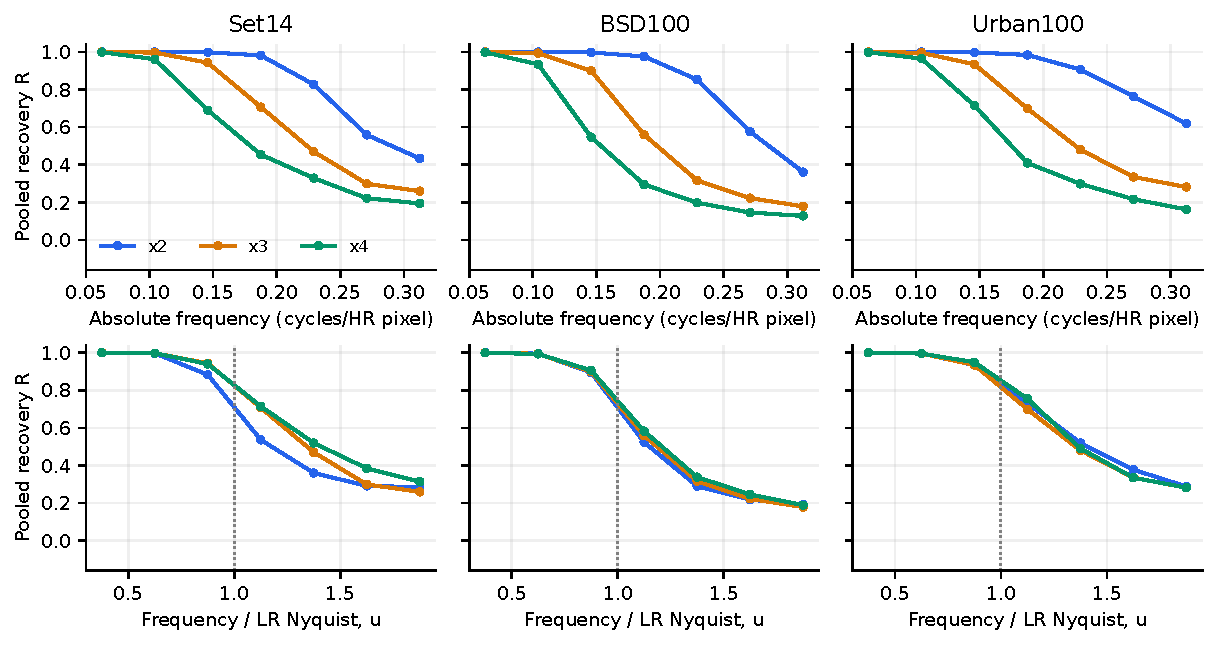
\includegraphics[width=.95\textwidth]{figures/l1-scale-recovery.pdf}
\caption{Scale-dependent recovery of SC-INR (seed1), from the saved L1 energy arrays. Top: fixed absolute-frequency bins. Bottom: the same measurement in LR Nyquist units $u=2s\nu$; the vertical line marks $u=1$. Curves use pooled energy ratios, not a mean of image-wise recoveries. The axes describe evaluated error and need not stay in $[0,1]$. Normalisation substantially reduces scale differences; Table~\ref{tab:l1-main} retains the Set14 threshold failure and all three-model results.}\label{fig:l1-main}
\end{figure*}

\paragraph{Content sensitivity.} A post-hoc leave-one-image-out check identifies barbara as the largest contributor to the Set14 discrepancy. Removing it reduces $D_{\rm in}$ to $.0361/.0298/.0300$ for LIIF/LTE/SC. For comparison, 200 fixed-seed samples of 14 images from the first 30 BSD100 images have respective maxima $.0392/.0378/.0388$. This diagnoses sensitivity of energy pooling to image content; it does not establish JPEG artefacts or a capacity mechanism. We retain the original failed cohort and criterion. Extrapolation and public-model checks likewise remain limited: the original outside-training-range criterion and public-model aggregate each pass only six of nine groups.

\subsection{Paired readout losses and coarse band ordering}\label{sec:readout-main}
The readout comparisons pair LTE with LTE-NoCell and SC-INR with SC-INR-NoSinc under the recovered matched training setup. Define
\begin{equation}\label{eq:loss}
L_b=R_b^{\rm full}-R_b^{\rm ablated}.
\end{equation}
Positive $L_b$ means the full readout improves recovery; negative values are retained. A paired training ablation measures the change between trained models, not the effect of deleting a component while holding all learnt weights fixed. LTE phase conditioning and SC sinc feature modulation are evaluated separately; neither is assumed to implement the same physical pixel integral.

The original F1 small-mismatch predictor $g(R)=R(1-R)^2$ fails the $.5$ correlation threshold for both architectures: $.411/.400$ with linear recovery, $.490/.492$ with network recovery. Cross-architecture loss ranking is high ($.985$), but magnitudes differ. For the correct SC pair, mean losses over $b_1/b_2/b_3$ are $-.0000142/+.0001368/+.0080551$; A-labelled cells average $-.0006091$, and $\times3$ $b_2$ averages $+.0010338$ (LTE: $+.0050$). Some SC cells improve after ablation, including Set14 $\times2$ $b_3$ ($-.03788$). High rank correlation therefore does not imply equal benefits or a common quantitative mechanism.

G1 tests a simpler predictor: the box-footprint versus point-sampling quantity $\epsilon(\nu)=1-\operatorname{sinc}(\nu_x)\operatorname{sinc}(\nu_y)$ gives fixed squared-band scores $(.00006,.00552,.07235)$. It was proposed after seed1 and frozen before seed2/3 evaluation. The full original protocol has been recovered and hash-verified. Table~\ref{tab:g1-main} reports all four confirmatory groups.

\begin{table}[t]\centering\small
\caption{G1: 27 cells per group. Average ranks handle the predictor's three tied band values. Adding $h(R)=R(1-2R)^2$ reduces correlation in every group.}\label{tab:g1-main}
\begin{tabular}{lccc}\toprule
Group & $\rho(\epsilon_b^2,L)$ & $\rho(\epsilon_b^2h(R),L)$ & $L_3>L_2$\\\midrule
LTE seed2 & .577 & .532 & 8/9\\
SC seed2 & .943 & .703 & 9/9\\
LTE seed3 & .676 & .643 & 8/9\\
SC seed3 & .885 & .804 & 9/9\\\bottomrule
\end{tabular}
\end{table}
The original ordering threshold passes in four of four groups; $L_3>L_2$ occurs in 34/36 settings. The additional recovery factor supplies no improvement under the frozen criterion. Because the three scores are strictly increasing, replacing them by band indices $(1,2,3)$ gives exactly the same average ranks and Spearman correlations. The test therefore supports coarse frequency ordering across these architecture--seed groups, with no advantage over that free baseline. It does not validate a gain-mismatch explanation, nor a precise loss amplitude. Saved pooled statistics and coverage are independently checked; G1 did not save per-image signal/error energy weights, so full independent repooling is unavailable.

\subsection{Scale marginalisation predicts ordering but not the ablated function}\label{sec:l2-main}
L2 asks whether a network without a scale readout behaves like the full model averaged over the training-scale inputs. At fixed coordinates and image features, we average predictions over 31 cell inputs corresponding to $s'\in\{1.0,1.1,\ldots,4.0\}$, obtaining $R_{\rm marg}$. The proposed loss is $L_{\rm pred}=R_{\rm full}-R_{\rm marg}$. The primary test covers the 27 $\times2/3/4$ cells; log-spaced queries and $\times8$ are secondary. The uniform scale average is an operational diagnostic, not a conditional distribution of scale given the LR image. This is a post-training diagnostic using HR truth, not a deployable LR-only rule.

\begin{table}[t]\centering\small
\caption{Complete L2 seed2/3 replication. Ratio is the median $L_{\rm pred}/L$ over $L>.005$. Similarity is the fraction of image--scale pairs where the ablated output is closer to the marginalised than the full output.}\label{tab:l2-main}
\begin{tabular}{lcccc}\toprule
Group & $\rho$ & Ratio & Similarity & $\rho-\rho_\epsilon$\\\midrule
LTE seed2 & .712 & .823 & .770 & +.130\\
SC seed2 & .755 & .581 & .689 & $-.142$\\
LTE seed3 & .954 & .833 & .748 & +.331\\
SC seed3 & .700 & .337 & .653 & $-.173$\\\bottomrule
\end{tabular}
\end{table}
Ordering passes in four groups and the magnitude interval $[.5,2]$ in three. Function similarity never reaches $.8$. Superiority over the simple footprint score by at least $.05$ occurs in two groups, below the required three; both are LTE. The cell-invariant ablation control passes in all four groups with maximum difference zero. Independent reconstruction from per-image signal/error energies reproduces the pooled values. The result supports empirical prediction of ordering, while rejecting function equivalence and a uniformly better account across architectures. G1 and L2 differ in crop, image count and colour aggregation, so their correlations are compared within their own protocols.

\subsection{Frozen-weight probes beyond band ordering}\label{sec:probe-main}
An additional frozen diagnostic separates the input observation, true output footprint and network cell hint on 72 known continuous fields and the already-seen barbara image (Appendix~\ref{app:readout-probes}). The final-RGB integral forecast reduces phase-held-out MAE against band index by 24.25\% and 22.42\% for SC-INR at input sizes 16/32, but recalls only 0/9 and 1/11 negative effects. It fails for LTE, and neither this forecast nor amplitude scaling passes the complete four-group criterion. These forecasts use known target truth and are not observation-only rules. Their positive SC result is therefore a limited magnitude diagnostic, not a reliable account of negative benefit.

Crossed target/hint scores retain both signs within every band. In barbara's $\times2$ high band, SC-INR's separately trained ablation gives a negative paired gain ($-.193296$), whereas native versus zero-cell conditioning of the same weights gives a positive gain ($+.009733$). These are distinct comparisons. The new probes delimit a common integral explanation; distribution and query-support differences prevent attributing their failures to architecture alone.

A separate prospective observation-only test uses 32 fixed calibration images and 12 new continuation evaluation images (Appendix~\ref{app:negative-readout}). SC has 14 harmful band effects: a bicubic-proxy forecast recalls 4/14, and adding proxy alignment to calibrated magnitude/spectrum features recalls 6/14, with worse balanced accuracy than the same ridge without alignment ($.568$ versus $.585$). All four candidate/model combined gates fail; LTE has only one harmful band row. A fixed equal-observation diagnostic has 27/64 active sign reversals, bounding this proxy without proving a general impossibility or justifying matched training.


\section{Checks and Boundaries Beyond ASISR}\label{sec:boundary}
The following completed experiments constrain interpretation of the ASISR baseline. Their full tables and protocols are supplementary; none supplies a nonlinear readout theorem or an adaptive INR selector.

Classical linear experiments show useful approximate cost ranking but numerical counterexamples and unsuccessful winner selection. The complete prospective G2 cohort chooses the same prior in 36/36 cases, trails frame cross-validation by $.112$ dB and costs 1.76 times as much. It establishes neither target-specific adaptation nor an INR selector. The full checks, original criteria and costs are retained in Appendix~\ref{app:guidance-summary} and the supplementary experiment tables. They constrain interpretation rather than extend the paper's central contribution.

\begin{table*}[t]\centering\small
\caption{Claim hierarchy retained in the baseline. Passing a weaker test does not upgrade a failed stronger one.}\label{tab:claims-main}
\begin{tabular}{p{.28\textwidth}p{.35\textwidth}p{.29\textwidth}}\toprule
Question & Complete evidence & Supported conclusion\\\midrule
Does normalisation reduce scale variation? & L1 improves 9/9; strict tolerance passes 6/9 & Useful normalisation; no universal collapse\\
Can a fixed band score order readout losses? & G1 ranks 4/4; adding recovery factor improves 0/4 & Same ranks as band index; no gain mechanism\\
Does scale averaging reproduce the ablation? & L2 ranking 4/4, magnitude 3/4; similarity 0/4 & Correlational prediction; no function equivalence\\
Is L2 better than the simpler predictor? & Improvement in 2/4, below required 3/4 & No general superiority\\
Does calibrated analysis adapt to each target? & G2 constant choice in 36/36; worse accuracy/cost than CV & Default improvement; no adaptive advantage\\\bottomrule
\end{tabular}
\end{table*}

\paragraph{Exploratory evidence retained separately.} Same-observation linear/FF controls on two already-seen images include reverse rankings. A common 32-image empirical evaluation law selects the same strong static prior; it does not isolate a nonlinear mechanism or demonstrate adaptation. An 8-point Gaussian example and the associated finite-sample confidence-set study concern fresh-draw population risk, not single-image safety; they remain classical illustrative material. EEG supplies only 200 calibration segments, with the 760-segment test archive missing. These results motivate scope restrictions rather than cross-modal or new-theory contributions.

\section{Limitations}\label{sec:limits}
\paragraph{Reference and numerical scope.} Linear optimality is conditional on the specified covariance, centring, operator and noise. The image-periodogram oracle is truth-dependent. E3's assumed variance, clipping, amplitude scaling and missing pixel/energy/residual archives limit its use to the recovered descriptive comparison. Exact matrix identities do not certify an approximate solver or a clipped output. E1 also has a native forward/inverse discretisation mismatch.

\paragraph{Empirical generalisation.} ASISR results cover a limited set of decoders, training recipes, datasets and three seeds. Bands and cells share images and are dependent. Similar recovery is not a Bayes limit or proof that more capable decoders cannot improve. Nyquist normalisation improves consistency but fails the original strict threshold in Set14; content sensitivity and readout losses remain empirically observed, not causal explanations.

\paragraph{Mechanism and guidance.} Classical scalar identities require fixed effective noise and cannot be substituted into a nonlinear network without further assumptions. G1 has identical Spearman ranks to band index and supports only coarse ordering; L2 fails function similarity and general superiority over a simpler predictor. Threshold sensitivity at $.1/.8$ remains untested. G2 covers one operator, one calibration and fixed noise draws; its constant selection and worse comparison to CV leave adaptive and computational benefits unsupported. No learned INR model-choice rule is established. Existing HR targets do not certify box-integrated truth, and paired retraining is not a fixed-weight intervention. The additional frozen-weight probes are restricted to known-law synthetic content, unsupported rectangular/zero-cell hints and one retrospective natural image. Their partial SC magnitude improvements miss negative benefits; numerical quadrature has eight unresolved rows and integrates a conditional reference rather than a certified physical point field. IPE-LIIF and Thera already cover integrated encoding and analytic filtering; a new readout contribution would require evidence beyond these principles. The additional observation-only comparison has just 12 fixed evaluation images and no added directional advantage over its norm/spectrum ridge. LTE supplies only one negative band row. Bicubic proxy error is prior-dependent, and 27 specific same-observation sign reversals delimit the fixed-weight decision without implying an all-estimator lower bound. No matched training is undertaken.

\paragraph{Preserved auxiliary evidence.} Supplementary controls use already-seen development images and single seeds. Their reverse rankings and static-baseline equivalence are retained. The Gaussian ambiguity example depends on the allowed estimator class; a restricted two-candidate regret bound is not an all-estimator reconstruction lower bound. Classical covariance-estimation and design tools are not claimed as new theorems. Calibration-only EEG does not supply independent cross-modal validation.

\section{Conclusion}
The paper baseline concerns scale-dependent frequency recovery and readout effects in ASISR. Nyquist normalisation reduces scale variation, and coarse readout-loss ordering replicates across two architecture pairs and two additional seeds. Stronger collapse, function-equivalence, quantitative mechanism and adaptive-selection claims remain unsupported by their respective tests. Covariance-conditioned linear references and classical mismatch costs help organise these observations, with their assumptions and numerical limits stated separately. Further innovation should be assessed against this preserved baseline rather than inferred from additional correlations or oracle comparisons.


\begingroup\small
\bibliographystyle{plainnat}
\bibliography{refs}
\endgroup

\clearpage
\appendix
\section*{Supplementary material}
Extended ASISR results and auxiliary experiments are followed by classical derivations, reproducibility limits and exploratory controls.
\section{Extended experiments and recovered protocols}\label{app:extended}

\paragraph{Protocol.} Confirmatory thresholds follow the recovered pre-registrations. Freezing is audited experiment by experiment: E2 windowing changed after a one-image pilot, G1 predictors were proposed after seed1, and exploratory analyses are not promoted to confirmation. Images are from
DIV2K validation (0801--0812) unless stated; $R_b$ uses each recovered protocol: F1/G1/E3 average RGB to grayscale, L2 pools RGB channel energies, and E1/D11 retain RGB metrics.
Exploratory analyses are labelled as such.

%-------------------------------------------------------------------
\subsection{The mismatch cost is predictable (E2)}\label{sec:exp-e2}

\paragraph{Setup.} 12 DIV2K images, five tasks (single image $\times2$,
$\times4$; sparse pixels 10\%, 25\%, 50\%). In each of the three bands we
multiply the true spectrum by $\kappa\in\{1/16,1/4,4,16\}$, reconstruct with a
GP (linear), and measure the lost recoverability in that band, giving 60
cells \src{E2§2}. Band energies are computed after a Hann window on
both signal and error; the window was not specified in the pre-registration
and was added after a one-image run showed boundary leakage (single-image
$\times4$ $b_3$ measured $R=0.56$ at 0.004\% transmittance). After the fix,
single-image $\times4$ $b_2$ measures $R=0.085$ against an a-priori 0.08
\src{E2§1}. Only the metric changed, not hypotheses or criteria.

\begin{table}[t]\centering\small
\caption{Original E2 reported criteria (60 cells, 12-image means)
\src{E2§2; E4-T1}.}\label{tab:e2}
\begin{adjustbox}{max width=\linewidth}\begin{tabular}{lcc}\toprule
Criterion & Threshold & Result\\\midrule
a. Spearman(band-avg.\ prediction, measured) & $\ge0.8$ & \textbf{0.90}\\
b. $R<0.3$: over-est.\ $>$ under-est. & $\ge80\%$ & 4/4\\
b. $R>0.7$: under-est.\ $>$ over-est. & $\ge80\%$ & 6/7\\
c. median $|$pred.$-$meas.$|$ & $\le0.05$ & 0.038\\
d. Spearman(a-priori prediction, measured) & $\ge0.7$ & 0.79\\
\bottomrule\end{tabular}\end{adjustbox}
\end{table}

\begin{table}[t]\centering\small
\caption{Original E2 measured / band-averaged predicted cost $\Delta$ (fraction of band
energy) \src{E2§3}.}\label{tab:e2cells}
\setlength{\tabcolsep}{3pt}
\begin{adjustbox}{max width=\linewidth}\begin{tabular}{lccccc}\toprule
Task, band & $R$ & $\kappa{=}\tfrac1{16}$ & $\tfrac14$ & 4 & 16\\\midrule
SI$\times2$ $b_2$ & .80 & .230/.402 & .047/.101 & .067/.031 & .165/.056\\
SI$\times2$ $b_3$ & .11 & .084/.097 & .044/.058 & .194/.380 & \textbf{1.370}/2.648\\
SI$\times4$ $b_2$ & .085 & .060/.074 & .029/.045 & .150/.336 & \textbf{0.933}/2.590\\
Sparse 10\% $b_2$ & .37 & .197/.291 & .072/.144 & .110/.302 & .586/.976\\
Sparse 25\% $b_2$ & .70 & .226/.430 & .068/.139 & .094/.074 & .473/.149\\
Sparse 50\% $b_2$ & .90 & .148/.264 & .036/.046 & .024/.009 & .064/.015\\
\bottomrule\end{tabular}\end{adjustbox}
\end{table}

\paragraph{Independent reimplementation (E2r).} A separate implementation
reproduces all 60 aggregated cells from 12 images and five tasks. Its
post-hoc cost ranking is .902528, reference-prior ranking .797188 and
median absolute error .035099 (maximum 1.8895). Asymmetry counts are 4/4
and 6/7; all four frozen thresholds pass. These are distinct rerun numbers,
not replacements for individual original cells in Tables~\ref{tab:e2}
and~\ref{tab:e2cells}. The high maximum error limits quantitative
interpretation despite the passed median threshold \src{E2r}.

\paragraph{Results.} All four pre-registered criteria hold
(Table~\ref{tab:e2}). For example, single-image $\times4$ $b_2$ has under-estimation cost $.060$ and over-estimation cost $.933$ for reciprocal factors $1/16$ and $16$; the latter exceeds the matched recovery $.085$ and hence is worse than zero band reconstruction
(Table~\ref{tab:e2cells}). In high-$R$ bands the direction reverses. In the reported near-zero-recovery cell (single image $\times4$ $b_3$), both evaluated finite mismatch factors incur small costs; this is not uniform over arbitrarily large factors \src{E2§3}.
The band-averaged prediction over-estimates large-$\kappa$ costs in the reported examples; this direction is not general. For
decimation, evaluating Eq.~\eqref{eq:delta} per frequency with
Eq.~\eqref{eq:alias} and energy-weighting reduces approximation error in the reported exploratory calculation (exploratory:
Spearman 0.99, median error 0.004; e.g.\ SI$\times4$ $b_2$, $\kappa=4$:
predicted 0.151, measured 0.150) \src{E2§4}.
The single counter-example to the asymmetry is sparse 10\% $b_1$ ($R=0.92$;
under 0.072 vs.\ over 0.110): random sampling spreads aliasing across bands,
outside the scalar model \src{E2§2}.

%-------------------------------------------------------------------
\subsection{Low-reference-recovery bands: similarities among evaluated ASISR decoders (M2, E3)}\label{sec:exp-c}

\paragraph{Setup.} We compare four trained decoders that share the
EDSR-baseline encoder and the LIIF training protocol (DIV2K, 1000 epochs,
scale range $\times1$--$\times4$, seed 1): LIIF, LTE, SC-INR-eq and
SC-INR without the sinc footprint readout. This early comparison is not a matched SC-INR/NoSinc ablation; the latter is evaluated separately in F1/G1
against two linear references, LMMSE with the generic spectrum and LMMSE with
the image's own (oracle) spectrum, on $256^2$ centre crops of the first 30
images of Set14, BSD100 and Urban100 \src{OUT7.1/h6c}.

\begin{table}[t]\centering\small
\caption{Single image $\times4$, $R_b$ measured on data
\src{OUT7.1/h6c}. Regime by $\Rlin$: $b_2$, $b_3$ are C. gen./orac.: LMMSE with generic/oracle spectrum; SC-eq/SC-ns: SC-INR-eq / SC-INR-nosinc.}
\label{tab:h6c}
\setlength{\tabcolsep}{3pt}
\begin{adjustbox}{max width=\linewidth}\begin{tabular}{llcccccc}\toprule
Set & band & gen. & orac. & LIIF & LTE & SC-eq & SC-ns\\\midrule
Set14 & $b_2$ & .16 & .25 & .56 & .57 & .57 & .56\\
 & $b_3$ & .09 & .09 & .20 & .20 & .20 & .18\\
BSD100 & $b_2$ & .13 & .22 & .38 & .38 & .38 & .38\\
 & $b_3$ & .06 & .06 & .13 & .13 & .13 & .11\\
Urban100 & $b_2$ & .11 & .27 & .50 & .50 & .51 & .51\\
 & $b_3$ & .02 & .03 & .14 & .14 & .15 & .13\\
\bottomrule\end{tabular}\end{adjustbox}
\end{table}

\paragraph{$\times4$.} In both regime-C bands the trained networks recover
more than the evaluated oracle-periodogram linear reference: 0.38--0.57 vs.\ 0.22--0.27 in $b_2$
(1.7--2.3$\times$) and 0.13--0.20 vs.\ 0.03--0.09 in $b_3$ (2--6$\times$)
(Table~\ref{tab:h6c}). This comparison is consistent with benefits from a learned prior, but does not prove that all linear models or all alternative priors fail on these images.
The four decoders differ by at most 0.02 in either band.

\paragraph{Across scale factors (E3).} We repeat the measurement at
$\times2$, $\times3$, $\times8$ (27 cells: 3 scales $\times$ 3 bands $\times$
3 datasets) with the same networks; $\times8$ is out of the training range
\src{E3}. Pre-registered results (Table~\ref{tab:e3}): the a-priori
$\Rlin$ ranks the measured generic-LMMSE recovery with Spearman 0.952; in
10/12 regime-C cells all four networks exceed the oracle LMMSE and differ by
at most 0.03; in 9/9 regime-A cells the best network is within 0.05 of the
oracle LMMSE (largest gap $+0.016$); generic-LMMSE recovery decreases
monotonically with scale in 9/9 band--dataset pairs. The descriptive reference labels change with scale: $b_2$ is A at $\times2$ ($\Rlin=0.92$), B at $\times3$ (0.42) and
C at $\times8$ (0.011); $b_1$ enters B at $\times8$ (0.79)
\src{E3-key}. In all 12 C cells every network exceeds the oracle
(by $+0.002$ to $+0.244$) \src{E4-T2}.

\paragraph{Scale collapse (L1, pre-registered).} The measurement hypothesis is that recovery is more consistent across scales when frequency is expressed relative to LR Nyquist, $u=2s\nu$, than in absolute frequency; this comparison does not identify an observation-only causal limit. On
$240^2$ crops of the first 30 images per dataset, we measure $R(u)$ in seven
$u$ bins at $\times2/\times3/\times4$ for LIIF, LTE and SC-INR (seed 1) and
take the median range across scales, $D_{\mathrm{in}}$ \src{L1L2}. The
linear control collapses ($D_{\mathrm{in}}$ 0.019 / 0.006 / 0.011 on Set14 /
BSD100 / Urban100). Binning by $u$ instead of $\nu$ shrinks the range by an
order of magnitude in 9/9 model--dataset groups (0.013--0.061 vs.\
0.31--0.46). The main criterion, $D_{\mathrm{in}}\le0.05$ in $\ge8/9$ groups,
fails: 6/9, with all three models on Set14 at 0.055--0.061 (BSD100 and
Urban100: 0.013--0.019). This exceeds both the seed noise floor (median range
across seeds 0.003--0.004) and the linear control; a post-hoc leave-one-image-out diagnostic identifies barbara as the largest contributor. Removing it gives $D_{\mathrm{in}}=.030$--$.036$, whereas 200 fixed-seed subsets of 14 images from the first 30 BSD100 images give maxima $.0378$--$.0392$. These descriptive checks retain the original failure and do not prove a JPEG or capacity mechanism. We found no consistent deviation outside the training range
($\times6/8/12$; $D_{\mathrm{out}}>D_{\mathrm{in}}$ in only 6/9), and the
public models generalise only partly (GSASR and Thera pass, ContinuousSR
fails; 6/9) \src{L1L2}. Above the LR Nyquist limit, our three decoders
exceed the generic linear estimate by $+0.18$ to $+0.40$ and show small differences in these evaluated cells \src{L1L2}.

\begin{table}[t]\centering\small
\caption{E3 pre-registered criteria \src{E3; E4-T1}.}\label{tab:e3}
\begin{adjustbox}{max width=\linewidth}\begin{tabular}{lcc}\toprule
Criterion & Threshold & Result\\\midrule
a. Spearman($\Rlin$, generic LMMSE) & $\ge0.8$ & 0.952\\
b. C: nets $>$ oracle, range $\le0.03$ & $\ge80\%$ cells & 10/12\\
c. A: best net $-$ oracle $\le0.05$ & $\ge80\%$ cells & 9/9\\
d. generic LMMSE monotone in scale & 9/9 & 9/9\\
e. (expl.) oracle$-$generic: B$>$A, B$>$C & -- & .078 vs .011/.040\\
\bottomrule\end{tabular}\end{adjustbox}
\end{table}


\paragraph{Recovered E3 implementation.} Prior simulation injects Gaussian noise with $\sigma=.002$; natural-image E3 injects none, while the GP uses assumed variance $\nu=10^{-5}$ as regularisation. Generic-prior amplitude is scaled using HR truth variance. The LR is clipped but the linear operator is not; prior-window bands include DC whereas natural-image bands exclude it. Recovery averages RGB to grayscale, rather than using luminance. Prior sampling averages three draws, not an exact covariance trace. Saved per-image bootstrap intervals concern an unweighted mean of recoveries, not the energy-pooled table statistic. Original archives do not retain predictions, observations, band energies or true CG residuals; the present independent audit reproduces scalar records and criteria, not pixel reconstruction or numerical optimality. These differences preclude a matched-noise or deployable training-free boundary claim.

\paragraph{Reading.} These evaluated networks have similar band recovery
in 10/12 low-reference-recovery cells at a .03 range threshold, but only
8/12 at .02. This does not establish a universal limit on decoder design,
and changing the learned prior or training recipe remains outside this
comparison. The oracle-periodogram estimate is a reference rather than a
certificate of optimal realised linear recovery.

%-------------------------------------------------------------------
\subsection{Spectral-prior effects under sparse observations (M3, M4)}\label{sec:exp-b}

\paragraph{Sparse pixels.} Sampling rates 5--50\%, DIV2K 0801--0812,
luminance; we compare linear estimation with the generic spectrum, with the
image's own spectrum, and DIP \citep{ulyanov2018dip} \src{OUT7.2/sp\_scan}. The true-spectrum linear estimator beats DIP at every rate
(26.39 vs.\ 25.19, 28.45 vs.\ 27.02, 32.66 vs.\ 30.84, 37.89 vs.\ 34.79\,dB at
5/10/25/50\%), and the generic spectrum trails it by 1.8--4.5\,dB
(Table~\ref{tab:sparse}). The space between the two linear estimators is the observed gap between these two evaluated linear references.

\begin{table}[t]\centering\small
\caption{Sparse-pixel reconstruction: $R_{b_2}$, $R_{b_3}$ and PSNR (dB) for
generic / true-spectrum linear / DIP \src{OUT7.2}.}\label{tab:sparse}
\setlength{\tabcolsep}{3pt}
\begin{adjustbox}{max width=\linewidth}\begin{tabular}{lccc}\toprule
Rate & $b_2$ & $b_3$ & PSNR\\\midrule
5\% & .17/.39/.16 & .10/.20/.05 & 24.59/26.39/25.19\\
10\% & .29/.56/.34 & .14/.31/.12 & 26.13/28.45/27.02\\
25\% & .59/.81/.69 & .29/.57/.38 & 29.27/32.66/30.84\\
50\% & .85/.95/.89 & .57/.82/.65 & 33.37/37.89/34.79\\
\bottomrule\end{tabular}\end{adjustbox}
\end{table}

\paragraph{1D EEG.} On 200 calibration segments of EEGMMIDB
\citep{schalk2009eeg,schalk2004bci2000} with 10/25/50\% of samples
kept, the spectral prior helps most in $\theta$/$\alpha$ at 10--25\% and
almost nowhere at 50\%, where most bands are already A; e.g.\ $\alpha$ at
10\%: linear interpolation .22, population-average spectrum .30, true
spectrum .47 \src{OUT7.3}. These are calibration-only numbers from the original report. The 760-segment test result has not been recovered and is not counted as confirmatory evidence here.

%-------------------------------------------------------------------
\subsection{Multi-frame SR across noise levels (E1)}\label{sec:exp-ab}

\paragraph{Setup.} DIV2K 0801--0812, $\times4$, $T=16$ shifted frames
synthesised neutrally (footprints integrated on the $512^2$ original, ground
truth by $2\times2$ averaging), known registration, RGB, PSNR with an 8-pixel
border crop; $\sigma_n\in\{0,0.005,0.01,0.02\}$ \src{E1}. Arms: a
multi-resolution grid field (mrgrid); least squares with TV (ls\_tv); a
SuperF-style Fourier-feature MLP (ff\_$\sigma$); GPs with Gaussian spectra
(gp\_gauss\_$\sigma$), power-law spectra (gp\_power\_$\alpha$) and the
image's own spectrum (gp\_oracle); bilinear. Paired bootstrap 95\% CIs over
images.

\begin{table}[t]\centering\small
\caption{E1: 12-image mean PSNR (dB), $T=16$ \src{E1§2,
e1\_result\_v2.json}.}\label{tab:e1}
\begin{adjustbox}{max width=\linewidth}\begin{tabular}{lcccc}\toprule
Arm & $\sigma_n{=}0$ & .005 & .01 & .02\\\midrule
mrgrid & 31.39 & 28.36 & 22.57 & 14.36\\
ls\_tv1e-4 & 31.16 & 27.37 & 21.24 & 13.78\\
ls\_tv1e-3 & 29.98 & 29.61 & 28.64 & 24.84\\
ff\_3 & 27.94 & 27.92 & 27.88 & 27.74\\
ff\_10 & 28.86 & 28.79 & 28.61 & 28.01\\
gp\_gauss\_30 & \textbf{31.62} & 27.73 & 26.65 & 25.56\\
gp\_power\_2.0 & 31.19 & 29.37 & 27.37 & 26.10\\
gp\_power\_2.5 & 29.62 & 29.36 & 28.65 & 27.45\\
gp\_power\_3.0 & 28.27 & 28.21 & 28.04 & 27.50\\
gp\_oracle & 29.91 & \textbf{29.70} & \textbf{29.25} & \textbf{28.35}\\
bilinear & 24.65 & 24.64 & 24.59 & 24.41\\
\bottomrule\end{tabular}\end{adjustbox}
\end{table}

\paragraph{Results.} An observed noise trend is qualitatively consistent with the scalar account, without identifying a corresponding fixed prior for the nonlinear arms: representations without spectral decay (mrgrid, weak TV) collapse
under noise, losing 17\,dB between $\sigma_n=0$ and $0.02$
(Table~\ref{tab:e1}), an empirical deterioration rather than a demonstrated over-estimation mechanism; the value of the true
spectrum over the best power-law GP grows with noise, $D$ from 0.33 to
0.85\,dB, difference $+0.51$ [0.13, 0.88] (P3 holds); and the winner moves
from a low-bias arm (gp\_gauss\_30) to gp\_oracle (P4 holds)
\src{E1§1}. At $\sigma_n=0$ a low-bias GP beats the best
Fourier-feature MLP by $+2.76$ [1.99, 3.56]\,dB.

Two pre-registered predictions fail \src{E1§1}. (P1) At
$\sigma_n=0.005$ low-bias representations no longer win: mrgrid $-$ ff\_10 $=
-0.43$ [$-1.01$, 0.14]\,dB; the switch happens earlier than predicted.
(P2) At $\sigma_n=0.02$ the generic power-law GP does not come within 0.6\,dB of
the oracle ($-0.85$ [$-1.10$, $-0.61$]). The winner margins at $\sigma_n=0$
and $0.005$ are not significant (+0.19 and +0.10\,dB, CIs include 0).

\paragraph{Retrospective discrepancy diagnosis.} The pre-registered prediction used one
zone label: at $T=16$, $R^{\mathrm{lin}}_{b_2}$ falls from 0.90 to 0.73 over
the noise range (Table~\ref{tab:map}), so $b_2$ is regime A at small noise and
low-bias arms were expected to win. It ignored each arm's mismatch $\kappa_b$
and ignored $b_3$. The GP-only D11 diagnostic below decomposes these discrepancies retrospectively; it does not identify the nonlinear arms' mechanisms. Two further
notes. P4's switch at 0.005 partly reflects gp\_oracle's numerical noise floor
at $\sigma_n=0$ (it is an oracle reference; covariance-conditioned optimality does not certify its realised per-image performance), so future switch predictions should compare practical
arms only \src{DER§2.2}. For the non-linear arms, mrgrid and ls\_tv1e-4 already
lose more at $\sigma_n=0.005$ than their noiseless lead over ff\_10, which is
the direct numerical reason P1 fails; their mechanism was not tested
\src{DER§2.2}.

\paragraph{Diagnostic on E1 (D11, pre-registered).} We stored per-frequency
error spectra of the GP arms on the E1 images and settings (CPU; the
non-linear arms mrgrid, ls\_tv and ff were not measured) \src{D11}. At
$\sigma_n=0.005$ the excess error of gp\_gauss\_30 over gp\_oracle splits
0.5\% / 44\% / 56\% over $b_1/b_2/b_3$. In $b_3$ the measured oracle
recovery is $R=0.22$ (regime B) with over-estimation $\kappa=4.5$; in $b_2$,
$R=0.80$ but $\kappa=16.4$ (Table~\ref{tab:d11}). The pre-registered rule
looked only at $b_2$; $b_3$ was already in regime B, and in $b_2$ a large
$\kappa$ is not free even at $R=0.8$, since the ``harmless over-estimation''
of regime A is the $R\to1$ limit. Pre-registered results: (a) the $b_3$ share
of gp\_gauss\_30's excess is 0.556 [0.464, 0.618], above 0.5 at the point
estimate but with a CI that includes it; (b) the band-wise predicted excess
$\sum_b E_b\,\Delta(R_b,\kappa_b)$ ranks the measured excess over 24 arm--noise
points with Spearman 0.856 [0.741, 0.918] (point threshold 0.8 holds, but the CI includes lower values); (c) it does
\emph{not} pick the best non-oracle GP arm (1/3 noise levels, threshold 2/3):
the top arms are close and the band-averaged form carries a band-aggregation error
(e.g.\ gp\_power\_2.0 at $\sigma_n=0.005$: predicted $1.40\times10^6$,
measured $3.9\times10^4$, unnormalised) \src{D11}. The concentration of excess
error on $R(\nu)<1/2$ frequencies (0.82 / 0.71 for the two wide arms vs.\ 0.18
for gp\_power\_3.0) has no discriminative value, because 78\% [74\%, 81\%] of
all frequencies satisfy $R(\nu)<1/2$ at this noise level; we do not use it
as evidence. So the band-wise cost $C(Q)$ (Eq.~\eqref{eq:crit}) ranks the GP arms but does
not select the winner; whether its a-priori version ranks equally well has not
been tested \src{DER§2.3}.

\begin{table}[t]\centering\small
\caption{D11: gp\_gauss\_30 vs.\ gp\_oracle, E1 multi-frame, $T=16$,
$\sigma_n=0.005$, 12-image mean \src{D11}.}\label{tab:d11}
\begin{adjustbox}{max width=\linewidth}\begin{tabular}{lccc}\toprule
Band & oracle $R_b$ & $\kappa_b$ & share of excess\\\midrule
$b_1$ & 1.00 & 1.02 & 0.5\%\\
$b_2$ & 0.80 & 16.4 & 44\%\\
$b_3$ & 0.22 & 4.5 & 56\%\\
\bottomrule\end{tabular}\end{adjustbox}
\end{table}

\paragraph{Bootstrap and diagnostic boundary.} The saved D11 script used
2,000 source-image resamples. We reproduced those draws and extended the
same paired procedure to the protocol's 10,000. The updated ranking CI is
[.741,.918]; an independent 10,000-draw image-cluster calculation gives
$b_3$ share [.464,.618]. Both condition on 12 images and fixed noise draws.
D11 uses truth-derived energy, oracle recovery and spectrum ratios;
its ranking is post-hoc and cannot establish a target-observation-only
selector. The cropped/windowed empirical $R_b$ and band ratios also do not
satisfy the exact scalar model by construction \src{CPU-10000}.

\noindent Non-linear arms (mrgrid, ls\_tv, ff) are covered only
qualitatively; $T=4/8$ (4 images) is descriptive only.


%-------------------------------------------------------------------
\subsection{Inside the network: SC-INR's footprint readout (F1)}\label{sec:exp-f1}

We study SC-INR's sinc feature modulation before its nonlinear RGB decoder and LTE's learned cell-phase conditioning, retaining positive and negative losses. Neither construction is assumed to integrate the final RGB field. F1 asks where in the band map this
component matters. We ablate it in two architecture pairs (LTE vs.\
LTE-NoCell; SC-INR vs.\ SC-INR-NoSinc) and measure the per-band loss
$L=R_{\mathrm{full}}-R_{\mathrm{ablate}}$ on 27 confirmatory cells
($\times2/\times3/\times4$ $\times$ 3 bands $\times$ 3 datasets), seed 1
\src{F1}. The pre-registered predictor is $g(R)=R(1-R)^2$, the
small-mismatch limit of Eq.~\eqref{eq:delta}.

\paragraph{Results (LTE pair).} $L$ is small on average in the high-reference-recovery cells: mean $L$ over
regime-A cells is 0.0000, versus 0.0050 at $\times3$ $b_2$ (regime B)
\src{F1; E4-T1}. The loss concentrates in $b_3$ at $\times2$--$\times4$
and $b_2$ at $\times4$, where $\Rlin$ is only 0.01--0.10 (regime C) but the
network recovers 0.13--0.56. The a-priori predictor fails:
Spearman$(g(\Rlin),L)=0.411<0.5$ (standard Spearman with average ranks for
ties). Using the network's own recovery raises it to 0.490, still below the
threshold \src{E4-T1}.

\paragraph{Results (SC-INR pair).} With the matched pair (SC-INR vs.\
SC-INR-NoSinc, same encoder), the coarse ordering is similar but the magnitude is smaller: the A-regime criterion
holds, the a-priori predictor fails (Spearman$(g(\Rlin),L)=0.400$), the
network-recovery predictor also stays below threshold (0.492), and the
per-cell losses of the two architectures have highly correlated ranks (Spearman 0.985)
\src{F1-corr2}. Mean $L$ in the A cells is -0.000609, versus 0.001034 at $\times3$ $b_2$, from the saved corrected table. All F1 numbers are seed 1 only; seeds 2/3
are evaluated under the G1 pre-registration below.


\paragraph{A closed-form band-order predictor (G1, completed).}
The box-footprint versus point-sampling quantity
$\epsilon(\nu)=1-\operatorname{sinc}(\nu_x)\operatorname{sinc}(\nu_y)$
provides three fixed band scores $(.00006,.00552,.07235)$. It was chosen
after seed1; only seed2/3 count toward confirmation. The original protocol
was recovered byte-for-byte and matched its frozen SHA256
(\texttt{548b26fe} prefix). Correctly paired HR256 evaluations contain
13 Set14, 30 BSD100 and 30 Urban100 images; $\times3$ uses LR85.
\begin{table}[t]\centering\small
\caption{Completed G1 confirmation; 27 aggregated cells per group.}
\label{tab:g1}
\begin{tabular}{lccc}\toprule
Group & $\rho(\epsilon_b^2,L)$ & $\rho(\epsilon_b^2h(R),L)$ & $L_3>L_2$\\\midrule
LTE seed2 & .577 & .532 & 8/9\\
SC seed2 & .943 & .703 & 9/9\\
LTE seed3 & .676 & .643 & 8/9\\
SC seed3 & .885 & .804 & 9/9\\\bottomrule
\end{tabular}
\end{table}
H-G1 passes in 4/4 groups (at least 3 require $\rho\ge.5$); H-G2
passes in 34/36 settings (threshold 26); H-G3 passes in 4/4:
$h(R)=R(1-2R)^2$ adds no improvement within the .05 allowance.
Replacing the three increasing scores by band index gives identical
Spearman ranks and correlations. This supports coarse frequency-band
ordering, not the functional form of the footprint score or a quantitative
gain mechanism. With only three distinct predictor values, tied average ranks
are essential. The linearised gain account was separately rejected by
L2b. Newly computed predictions were not used to tune the thresholds
\src{G1-20261008}.

\paragraph{Predicting the loss from the full model (L2, pre-registered).}
One account is that the cell or footprint input tells the
decoder the scale factor, so a model without it behaves like the full model
averaged over the training scales. We test this without training: average
the full model's output over cells corresponding to $s'\in\{1.0,1.1,\dots,4.0\}$
and predict the ablation loss as $L_{\mathrm{pred}}=R_{\mathrm{full}}-R_{\mathrm{marg}}$
on the 27 F1 cells, seed 1 \src{L1L2}. The ranking matches:
Spearman$(L_{\mathrm{pred}},L)=0.822$ (LTE) and 0.824 (SC-INR), against
0.40--0.49 for the zone predictors of F1 and $+0.147/+0.149$ above the
footprint gain $\epsilon_b^2$ (0.676 on this evaluation) \src{L1L2}; with
log-uniform $s'$ it is 0.805/0.803. Two pre-registered criteria fail. The
magnitude matches only at $\times4$ and above: the median
$L_{\mathrm{pred}}/L$ is 0.59 (LTE) and 0.36 (SC-INR), outside $[0.5,2]$ for
SC-INR, because at $\times2/\times3$ the ablation loses more than
marginalisation predicts (e.g.\ BSD100 $\times3$ $b_3$: 0.038 vs.\ 0.008).
The ablated output is closer to the marginalised than to the full output in
73.9\% / 69.4\% of image--scale pairs (threshold 80\%), rising with scale
(LTE: 58\% at $\times2$, 99\% at $\times8$) \src{L1L2}. So the ablation loss can be predicted after the fact
from the full model's cell average, consistent with the readout supplying
scale information at large scale factors; at small scale factors the ablation
loses more than that, and the tested scalar predictors do not establish function equivalence
\src{DER§3.4}. This is correlational evidence; an isolated scale-information intervention has not been evaluated.

\paragraph{Completed L2 seed2/3 replication.}
All four frozen groups are now evaluated at HR240 (14/30/30 images), with
31 linear and 31 log-spaced cell queries. The primary 27 cells exclude
$\times8$. Independent recalculation from per-image signal and error
energies reproduces all pooled values.
\begin{table}[t]\centering\small
\caption{L2 replication. Ratio is median $L_{\rm pred}/L$ for $L>.005$;
similarity is the fraction closer to marginal than full output.}
\label{tab:l2multi}
\begin{tabular}{lcccc}\toprule
Group & $\rho$ & ratio & similarity & $\rho-\rho_\epsilon$\\\midrule
LTE seed2 & .712 & .823 & .770 & +.130\\
SC seed2 & .755 & .581 & .689 & $-.142$\\
LTE seed3 & .954 & .833 & .748 & +.331\\
SC seed3 & .700 & .337 & .653 & $-.173$\\\bottomrule
\end{tabular}
\end{table}
Under the original at-least-3/4 rule, H2a ordering passes 4/4 and H2b
magnitude passes 3/4. H2c function similarity passes 0/4 (threshold .8),
and H2d superiority over $\epsilon_b^2$ passes 2/4 (required improvement
.05); both fail the at-least-3/4 hypothesis criterion. The advantage occurs
only in LTE. H2z's cell-invariant ablation
control passes 4/4 with maximum difference zero. G1 and L2 use different
crops and pooling; their rows cannot be interchanged. These findings do
not establish that removing the readout produces the scale-marginalised
function, or that scale marginalisation is the best cross-architecture
mechanistic account \src{L2-20261008}.

%-------------------------------------------------------------------
\subsection{Prospective guidance: independent calibration (G2)}\label{sec:g2}
\paragraph{Frozen setup.} We test eight fixed GP spectra: Gaussian widths
$3,10,30,60,128$ and power-law exponents $2,2.5,3$. The default is
$1/f^2$. DIV2K training images 0001--0032 calibrate a unit stationary
covariance; 0801--0812 are development images. The complete target cohort
is 0813--0824 at $\sigma_n=.005,.01,.02$ (36 cases). These targets were not
used to develop this selector; they are not claimed to be globally unseen
in all earlier research. Matched $y=Ax+\epsilon$ uses HR256, $\times4$,
16 registered frames, eight footprint subsamples per axis and a 512 field.
RGB PSNR uses an eight-pixel crop and unclipped predictions. This controlled
geometry differs from E1's native forward model \src{G2-protocol}.

\paragraph{Observation-only rules.} All candidates share a contrast
estimate from noise-corrected observation energy and independent
calibration probes. Analysis selects the minimum expected cropped MSE
under the calibrated covariance, estimated by four common Gaussian probes
with physical noise and the observed-mean intercept. This is a plug-in
reference risk, not an unbiased target-risk estimate. Four-fold CV holds
out frames by index modulo four and estimates contrast from training frames
only. Each method refits its chosen prior on all frames. Each selector has
32 fits, but analysis uses full frames and CV uses 12: equal fit counts do
not imply equal cost. All 36 choices and chosen outputs were SHA-frozen
before scoring opened target truth. Double-precision PCG permits 4000
iterations and requires a freshly evaluated relative residual below
$10^{-5}$. Earlier development failures are retained; no target cases were
removed. All 36 completed with no failures; 2592 saved selection/evaluation
solver certificates pass, with maximum 3134 iterations \src{G2-audit}.

\begin{table*}[t]\centering\small
\caption{Complete G2 cohort. Gain is relative to fixed $1/f^2$;
95\% intervals use 10,000 bootstrap draws of 12 image clusters, averaging
three noises within each image. Regret is against the best of the eight
fixed candidates scored after freezing. Costs include common contrast
preparation, all selector fits and the chosen final fit, once per deployed
policy; shared fits are not added twice to actual experimental spending.
Calibration overhead is reported separately.}\label{tab:g2}
\begin{adjustbox}{max width=\textwidth}\begin{tabular}{lccccc}\toprule
Rule & Mean gain [95\% CI], dB & Regret mean/median/p90, dB & Worst gain, dB & $>1$ dB loss & Cost, s\\\midrule
Default & 0 & 1.219 / 1.064 / 1.801 & 0 & 0/36 & 160.5\\
Analysis & 1.105 [.726, 1.504] & .114 / 0 / .134 & $-.152$ & 0/36 & 8466.8\\
Four-fold CV & 1.217 [.754, 1.796] & .002 / 0 / 0 & 0 & 0/36 & 4821.7\\\bottomrule
\end{tabular}\end{adjustbox}
\end{table*}

\begin{figure*}[t]\centering
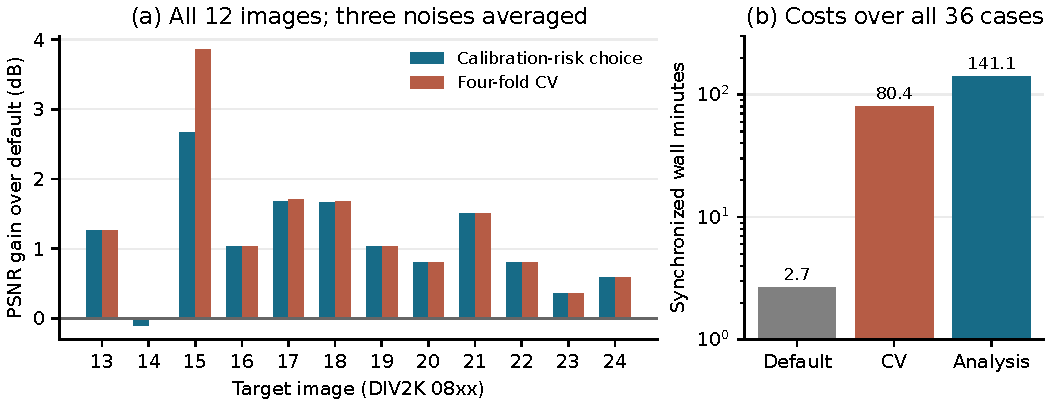
\includegraphics[width=\textwidth]{figures/guidance-results.pdf}
\caption{G2 complete-cohort gains and costs. (a) Every target image is
shown; averaging three noise settings does not create three independent
image replicates. (b) Synchronized wall time of common preparation,
selection and final fits on the same A800, on a log axis; this is not GPU
busy time. The analysis rule chooses power exponent 2.5 in all 36 cases,
so its gain does not establish instance-specific adaptation.}\label{fig:g2}
\end{figure*}

\paragraph{Results and counterexamples.} Analysis improves the default by
$1.105$ dB [.726, 1.504], with no $>1$ dB degradations, passing the
predeclared default-improvement gate (positive lower interval bound and
at most 5\% severe degradations). Its gains at the three noises are
$1.247,1.124,.945$ dB. CV improves the default by $1.217$ dB. The paired
analysis-minus-CV gain is $-.112$ dB [$-.313,-.002$], and analysis costs
1.76 times CV. The predeclared superiority-at-no-greater-cost gate fails
on both gain and cost. The frozen summarizer additionally requires zero
selection failures for that gate; there are none, so this extra restriction
does not change the conclusion \src{G2-result; G2-audit}.

Analysis chooses $1/f^{2.5}$ in 36/36 cases, whereas CV chooses exponents
2/2.5/3 in 3/27/6 cases. They hit the eight-candidate oracle in 25/36 and
34/36 cases respectively. Analysis loses to the default on image 0814 at
all three noises, worst $-.152$ dB; its largest oracle regret is 1.248 dB
on 0815 at .01 noise. A retrospective fixed-$1/f^{2.5}$ replay has
identical outputs to analysis, with common preparation and final fits
costing 194.6 s. This algebraic/cache identity is an interpretation of the
completed results, not an added confirmatory baseline or a new default
chosen before this test. The experiment does not isolate a benefit of
target-specific analytical selection \src{G2-audit}.

\paragraph{Full cost and practical reading.} Analysis and CV require
$5.065\times10^{12}$ and $3.222\times10^{12}$ interpolated points. Peak
recorded allocated memory is .488 GB. Calibration takes 3.0 s separately;
the actual resource ledger records 14,346.6 s of GPU-phase invocation wall
time, including the experiment's selection and oracle scoring, within the
24-hour budget. These timings depend on the shared-server load and are
not a benchmark of exclusive-device speed. Independent CPU audits reproduce
statistics and costs; all 78 cached chosen predictions were re-scored
from RGB pixels. Uncached candidate predictions were not retained, so
their oracle scores were audited from saved MSE and convergence records,
without an independent GP rerun. In this task, calibrated analysis finds
a better prior than the specified default, but frame-holdout CV adapts
more effectively and costs less. We therefore retain the analysis as a
conditional diagnostic, not a demonstrated cheap replacement for CV or
a neural-architecture selector \src{G2-audit}.

\section{Auxiliary guidance boundary summary}\label{app:guidance-summary}
The following account is preserved from the previous main text; it is not an additional ASISR contribution.
\paragraph{Linear mismatch checks.} E2 uses 12 DIV2K images, five tasks, three bands and four mismatch factors. An independent implementation reproduces all 60 aggregated cells: cost ranking $.903$, generic-reference ranking $.797$, median absolute error $.0351$, but maximum error $1.8895$. Low/high-recovery asymmetry counts are 4/4 and 6/7. Windowing was added after a one-image pilot, so the metric was not wholly specified before seeing data. Approximate cost ranking is stronger than its numerical accuracy; the original and rerun values remain distinct.

\paragraph{Oracle diagnosis versus feasible selection.} In sparse reconstruction the true-spectrum linear reference exceeds DIP at all four sampling rates, while the generic linear estimator trails DIP at all four. This is an oracle gap, not evidence that a deployable generic GP beats DIP. In multi-frame E1, two of four original switching predictions fail. D11's truth-derived band cost ranks 24 arm--noise points with $\rho=.856$ (10k image-bootstrap interval $[.741,.918]$), but picks the best non-oracle arm at only one of three noise levels. Rank correlation does not establish reliable winner selection.

\paragraph{Frozen prospective guidance.} G2 uses an independent 32-image calibration and a complete, frozen 12-image by three-noise cohort, choosing among eight fixed linear GP spectra before reading target truth. Analysis improves the specified power2 default by $1.105$ dB (image-cluster 95\% interval $[.726,1.504]$), but all 36 choices are power2.5. It trails four-fold frame CV by $.112$ dB (interval $[-.313,-.002]$) and costs $8466.8$ versus $4821.7$ seconds. A fixed power2.5 reconstruction would give identical outputs; its $194.6$-second retrospective cost excludes the work needed to choose that static prior. It is not a new confirmatory baseline or a selection speedup. The test does not establish target-specific adaptation, a cost advantage or INR architecture selection.


\section{Frozen-weight readout diagnostics}\label{app:readout-probes}
\paragraph{Question and separation.}
G1's three tied scores cannot distinguish a footprint formula from band index. We therefore freeze an additional diagnostic of effect magnitude and sign, separating the input measurement $A$, true target measurement $Q_h$, and decoder hint $c$. These probes neither retrain a decoder nor validate a deployable selector.

\paragraph{Known continuous targets.}
The field is $x(q)=.5+.25\cos(2\pi k(d_yq_y+d_xq_x)+\phi)$ on the unit square. Input box averages are evaluated analytically on $n\times n$ grids, with $n=16,32$, $k=4,6,10,14,18,26$, $d=(1,0),(0,1),(1,1)$ and $\phi=0,\pi/2$: 72 inputs. We query the central $32\times 32$ positions of a 64-grid, using four box sizes $(1,1),(2,1),(1,2),(2,2)/64$. For each input the observation, encoder features, weights and query centres remain fixed. The target transfer is $T_h=\operatorname{sinc}(kd_yh_y)\operatorname{sinc}(kd_xh_x)$. The evaluated LTE snapshot has no cell clamp, unlike the clamp described in the original LTE paper. All synthetic content differs from natural-image training; zero-cell and rectangular hints additionally differ from isotropic training support.

\paragraph{Reference field and forecasts.}
Let $F_0=F_\theta(y,q,0)$ and $F_c=F_\theta(y,q,c)$. $F_0$ is a zero-cell conditional reference, not a certified physical point field. With $S_h=\operatorname{mean}[(Q_hx-.5)^2]$, the signed gain is
\[
 G_{h,c}=\frac{\operatorname{MSE}(F_0,Q_hx)-\operatorname{MSE}(F_c,Q_hx)}{S_h}.
\]
For matched $c=h$, phase-zero data calibrate a band-median baseline and an affine fit in $(1-T_h)^2$; the fixed phase-$\pi/2$ grid evaluates them. Two stronger forecasts substitute either $.5+T_h(F_0-.5)$ or a numerical final-RGB integral $Q_hF_0$ for $F_h$. Both use the known target law for error scoring and are oracle diagnostics. Amplitude scaling also scales the reference's nuisance errors; it is not an exact filter of the true signal. Four- and eight-node midpoint rules per axis are retained. A row is numerically resolved only if their raw MSE difference is at most $10^{-5}$ and at most $.1$ of the native--eight-node discrepancy; this is a refinement check, not an integration certificate.

\paragraph{Frozen criteria and crossed hints.}
Each stronger forecast must reduce MAE by at least 20\% against both simple baselines in all four model--input-size groups, with active sign accuracy and negative recall at least $.75$. Active effects have $|G|>.001$; negative recall requires at least eight negative scoring rows. Integral forecasts additionally require all evaluation rows to be resolved. Footprints are correlated rows, not independent replicas. An add-on frozen before the first metric read crosses all four hints with all four true targets, reusing the saved predictions: 2304 scores, with no fitting or additional inference. Matching is evaluated against all four hints with raw-MSE tie tolerance $10^{-12}$; this ranking uses target truth.

\begin{table*}[t]\centering\small
\caption{Complete held-phase diagnostic: 72 correlated scores per group. MAE measures normalised gain. B: calibrated band median; F: affine footprint baseline; S: known-law amplitude scaling; Q: known-law numerical final-RGB integral. Q sign accuracy uses active effects; negative recall retains its full denominator. All stronger-candidate gates fail.}\label{tab:probe-prediction}
\begin{tabular}{lrrrrrrr}\toprule
Group & B MAE & F MAE & S MAE & Q MAE & Q sign & Q negative recall & Resolved\\\midrule
LTE16 & .13285 & .12838 & .23579 & .16820 & .2174 & 2/54 & 72/72\\
LTE32 & .28486 & .34996 & .33613 & .25082 & .5455 & 8/37 & 71/72\\
SC16 & .03223 & .04525 & .12427 & .02442 & .8163 & 0/9 & 72/72\\
SC32 & .23341 & .31576 & .27068 & .18108 & .8305 & 1/11 & 69/72\\\bottomrule
\end{tabular}
\end{table*}

\paragraph{Complete prediction results.}
Amplitude scaling and the integral forecast each pass zero of four complete group gates (Table~\ref{tab:probe-prediction}). SC's integral forecast improves MAE over both baselines by at least 20\% in both groups; its negative recall nevertheless fails. Positive cases comprise 40/49 and 48/59 active SC scores, so high sign accuracy alone can obscure failure on negatives. Its within-band rank correlations are $.690/.535/.727$ at $n=16$ and $.946/.797/.776$ at $n=32$. These finer correlations do not repair the failed criteria. LTE16's integral forecast worsens MAE relative to both simple baselines; LTE32 improves over band index by only 11.95\%, with sign accuracy $.5455$ and negative recall 8/37. Amplitude scaling fails magnitude and negative-recall requirements.

The fixed-grid cluster resampling intervals for the integral forecast's paired MAE difference against band index are $[-.02778,.00863]$ (SC16) and $[-.13611,.01639]$ (SC32), both crossing zero. Against the affine footprint baseline they are $[-.04386,-.00011]$ and $[-.22639,-.05053]$. These are sensitivity intervals on the fixed grid, not population confidence intervals. SC16's negative-recall resampling has two undefined draws out of 2000; both are retained as missing denominators. Across both phases 568/576 rows meet the refinement rule. The eight unresolved rows all have $n=32,k=14,d=(1,1)$: LTE square 2 and SC vertical/horizontal/square 2 in each phase. No rows are discarded. Median native--integral discrepancy divided by $S_h$ is $.03922/.06790$ for LTE16/32 and $.00131/.01324$ for SC16/32. Thus native conditioning differs from the numerically integrated reference on resolved rows, without certifying physical point readout \src{READOUT-20261011}.

\paragraph{Crossed target/hint counterexamples.}
Matched hints are among the minimum-MSE hints in 18/72, 21/72, 19/72 and 16/72 held-phase targets for LTE16/32 and SC16/32. This is not a comparison to a random policy, and mismatched hints performing better alone does not disprove integration: reference bias can change the best scored hint. Each group has both active signs within all three bands even when only matched hints are retained. Same-input, same-target hint changes also reverse the sign in 32/72, 48/72, 16/72 and 26/72 target groups, respectively (descriptive post-scoring counts with the frozen $.001$ margin). For example, LTE16's horizontal $k=10,\phi=\pi/2$ input and square 1 target have gain $-.19418$ for the square 1 hint and $+.06847$ for the vertical hint. These are training-support diagnostics, not a recommended choice of a physically incorrect footprint. Directional preference is not equivalent to target matching: swapping the true vertical/horizontal target changes the better equal-area hint in only 4/18 held-phase inputs for LTE32 and zero for the other groups \src{READOUT-CROSS-20261011}.

\paragraph{Negative-effect check and audit limits.}
For $e=F_0-Q_hx$ and $d=F_c-F_0$, $G=-(\operatorname{mean}(d^2)+2\operatorname{mean}(ed))/S_h$. This exact post-hoc identity distinguishes change energy from error alignment; it supplies no prospective predictor. The already-seen barbara image at $\times 2/4$ separately compares same-weight zero-cell conditioning and independently trained ablations. Its HR256 target is a discrete image, not box-integrated truth. Raw RGB errors and RGB-mean Fourier bands are primary, with clipped outputs reported separately. Independent audits re-score the saved outputs without importing the model implementation; they do not independently reimplement the network. Bootstrap resampling of 18 fixed frequency/direction clusters quantifies grid sensitivity, not natural-image generalisation.

\begin{table*}[t]\centering\small
\caption{All retrospective barbara bands. Paired gain compares separately trained full/ablated models; fixed gain compares native/zero-cell hints of the same full weights. In Fourier bands fixed gain is alignment minus change energy. Raw and clipped scoring agree here. These rows are not new natural-image tests.}\label{tab:probe-natural}
\begin{tabular}{lrrrr}\toprule
Model/scale/band & Paired gain & Fixed gain & Change energy & Alignment\\\midrule
LTE2 b1 & .000032 & .000817 & .000737 & .001555\\
LTE2 b2 & $-.146774$ & $-.015884$ & .027172 & .011288\\
LTE2 b3 & $-.100059$ & $-.004291$ & .018503 & .014212\\
SC2 b1 & .000060 & .000220 & .000170 & .000390\\
SC2 b2 & $-.264597$ & $-.006248$ & .003483 & $-.002765$\\
SC2 b3 & $-.193296$ & .009733 & .009779 & .019512\\
LTE4 b1 & $-.000004$ & .000236 & .000220 & .000456\\
LTE4 b2 & $-.001428$ & .012507 & .012330 & .024837\\
LTE4 b3 & .000982 & .002128 & .001354 & .003483\\
SC4 b1 & .000016 & .000006 & .000003 & .000009\\
SC4 b2 & $-.002644$ & .000363 & .000242 & .000605\\
SC4 b3 & .000805 & $-.000692$ & .000251 & $-.000440$\\\bottomrule
\end{tabular}
\end{table*}

SC's $\times 2$ high-band paired gain is $-.193296$, close to the original saved value $-.193291$ (maximum difference across its six historical bands $5.76\times 10^{-6}$, with CPU/GPU numerical paths differing). The same-weight gain is instead $+.009733$. Its mid-band fixed loss is $-.006248=-.002765-.003483$: both adverse alignment and change energy contribute. LTE2's mid-band alignment is positive but smaller than change energy, also yielding a loss. These decompositions calculate what happened; they do not explain prospectively why the learned change aligns this way \src{READOUT-20261011}.

\paragraph{Freeze, failures and full cost.}
All 74 inputs and 152 prediction files were frozen before truth scoring, including 48,709,632 RGB query positions. The fixed 2400-second wall/phase budget completes in 1376.925 seconds; the full launcher records 1377.305 seconds including teardown. CPU user/system time is 4501.156/601.088 seconds, peak recorded RSS 731.3MiB. CPU uses four threads and nice 10; training and GPU processes are zero. A backend segmentation fault in the first preflight and a missing timing executable in an earlier launcher are retained. Disabling MKLDNN passes a distinct 20.51-second preflight before the formal launch; neither the failed roots nor this preflight contributes to formal scores.

The independent saved-output audit verifies 148 input hashes, 152 prediction hashes, 41 frozen source records and four checkpoint identities, recomputing 576 synthetic and 24 natural rows with maximum difference $1.78\times 10^{-15}$ in 1.29 seconds. Cross scoring takes $.704$ seconds, and its independent 2304-row reimplementation takes $.626$ seconds, with maximum difference $3.55\times 10^{-15}$. The complete archive is verified after download. Freeze timestamps and inspected dataflow document artifact order, not an instrumented proof of every filesystem read. No training is initiated on these results: magnitude improvement in two SC groups leaves negative-benefit prediction and a shared quantitative mechanism unsupported.

\subsection{Observation-only prediction of harmful readout}\label{app:negative-readout}
\paragraph{Falsifiable hypothesis.}
A readout change can harm reconstruction either because it points away from the target or because its squared magnitude exceeds the improvement from alignment. The previous truth-based decomposition does not predict this direction. For a target proxy $b=B(y)$ and fixed outputs $p=F_0(y)$, $h=F_c(y)$, let $d=h-p$. We test the observable forecast
\[
 \widehat G=2\operatorname{mean}[(b-p)d]-\operatorname{mean}(d^2).
\]
For the raw actual gain $G=\operatorname{MSE}(p,t)-\operatorname{MSE}(h,t)$,
\[
 G-\widehat G=2\operatorname{mean}[(t-b)d].
\]
These are classical quadratic identities, not a new risk estimate. In particular, a small proxy error alone is insufficient if it couples to $d$. Our falsifiable prediction is that proxy alignment adds sign information beyond band, scale and magnitude/spectrum features, and that its use reduces the full-RGB loss of a policy choosing native versus zero-cell output.

\paragraph{Calibration and prospective comparison.}
We freeze DIV2K training images 0001--0032 for calibration and validation images 0825--0836 for evaluation, using centre HR128 crops, bicubic antialiased LR at $\times2/4$, no injected noise, and the same inherited LTE/SC epoch-1000 weights. The evaluation images were not scored in our earlier continuation cohorts; this does not establish that they were globally unseen during the inherited model development. Native square cell $1/128$ and zero-cell queries share LR, weights and centres. HR is the original discrete target. The proxy is raw bicubic upsampling of LR, not inversion of a box operator. All errors are unclipped RGB; a four-pixel shave gives a $120\times120$ region. Three per-channel Fourier bands use Chebyshev radius $[0,1/8),[1/8,1/4),[1/4,.5001)$, excluding DC; full-RGB loss includes DC and is scored separately. The normaliser $Z$ is the cropped proxy's mean channel-centred variance, floored at $10^{-8}$, never test truth energy.

Controls are always enabling/disabling the change, a calibration scale/band median, change energy alone, and a calibrated norm/spectrum ridge. This ridge uses scale/band indicators, log-normalised change/reference/proxy energy, LR gradient, spectral centroid and entropy. A directional ridge adds just the signed proxy-alignment feature to the same basis. Both use calibration-only standardisation, unpenalised intercept and fixed ridge penalty one, without hyperparameter search. The two candidates are the unfitted proxy forecast and directional ridge; neither is selected post-test. Calibration truth fits coefficients only, with no SR network optimisation. All evaluation predictions, coefficients and forecasts are SHA-frozen before evaluation truth is opened for scoring. Preparation necessarily reads HR to form LR; the freeze documents prediction/scoring order, not absence of all historical truth access.

\paragraph{Predetermined decision criteria.}
Raw effects with $|G|\le10^{-8}$ remain in the ledger but do not enter sign rates. Each model has 72 correlated band scores and 24 full-RGB decisions from 12 images. A candidate needs at least 12 negative rows spanning six images, negative recall $\ge.75$, precision $\ge.6$, false-positive rate $\le.25$, and balanced accuracy at least $.05$ above every control. Every paired image-cluster bootstrap interval must have positive lower bound for this accuracy difference. A full-RGB policy uses native output only for a positive forecast; its paired MSE reduction must likewise have positive lower bound against every control. Both classification and policy requirements must pass. We retain all 10,000 fixed-seed resamples, including undefined class denominators. These marginal intervals are not a simultaneous 95\% guarantee, and correlated bands/scales do not increase the independent image count. The forecaster needs both decoded outputs, so its cost includes that additional query rather than claiming pre-inference guidance.

\paragraph{Equal-observation diagnostic.}
Sixteen fixed axis-aligned periodic pairs use $n=16$ with low frequency $k=3,5$, or $n=32$ with $k=9,13$, on both axes and phases $0,\pi/4$. The high member has frequency $n-k$, amplitude $.25$ and phase $\pi-\phi$; the low member has amplitude $.25k/(n-k)$ and phase $\phi$. Their input box averages coincide, and one float32 observation and model inference serve both truths. The observable periodic proxy divides principal-mode input sinc transfer and applies each target's sinc transfer, retaining midpoint phases and dropping Nyquist rows/columns. Targets are square $1/64$ and $2/64$ footprints. Thus each pair has an identical forecast, while its scored effects need not coincide. Actual sign reversals are not guaranteed or used to select pairs; unchanged signs are retained. In general $Av=0$ changes the gain by $2\operatorname{mean}[(Q_hv)d]$, so spectral ambiguity alone need not imply ambiguity of this particular decision. This is a task-specific diagnostic, not an all-estimator impossibility theorem.

\begin{table*}[t]\centering\small
\caption{Complete prospective sign comparison. LTE has only one negative band row in one image; SC has 14 in nine images. All 72 rows per model are active. TP/negative is harmful-effect recall; FP/positive is rejection of useful changes. BA is balanced accuracy and normalised MAE uses observable $Z$. These dependent rows do not constitute 72 independent images. Neither candidate passes.}\label{tab:negative-sign}
\begin{tabular}{llrrrrr}\toprule
Model & Forecast & TP/negative & FP/positive & Precision & BA & MAE/$Z$\\\midrule
LTE & Enable & 0/1 & 0/71 & -- & 0.500 & -- \\
LTE & Disable & 1/1 & 71/71 & 0.014 & 0.500 & -- \\
LTE & Band median & 0/1 & 0/71 & -- & 0.500 & 0.00556 \\
LTE & Energy only & 1/1 & 71/71 & 0.014 & 0.500 & 0.01152 \\
LTE & Norm/spectrum ridge & 1/1 & 11/71 & 0.083 & 0.923 & 0.00187 \\
LTE & Proxy & 1/1 & 57/71 & 0.017 & 0.599 & 0.01599 \\
LTE & Directional ridge & 1/1 & 11/71 & 0.083 & 0.923 & 0.00192 \\
SC & Enable & 0/14 & 0/58 & -- & 0.500 & -- \\
SC & Disable & 14/14 & 58/58 & 0.194 & 0.500 & -- \\
SC & Band median & 0/14 & 0/58 & -- & 0.500 & 0.00206 \\
SC & Energy only & 14/14 & 58/58 & 0.194 & 0.500 & 0.00420 \\
SC & Norm/spectrum ridge & 6/14 & 15/58 & 0.286 & 0.585 & 0.00117 \\
SC & Proxy & 4/14 & 15/58 & 0.211 & 0.514 & 0.00341 \\
SC & Directional ridge & 6/14 & 17/58 & 0.261 & 0.568 & 0.00124 \\
\bottomrule\end{tabular}\end{table*}

\paragraph{Complete held-out results.}
The two candidates pass zero of four model/candidate combined gates. SC supplies 14 harmful band effects across nine images, meeting the denominator requirement, yet proxy recall is 4/14, precision 4/19 and BA $.51355$. Norm/spectrum ridge attains 6/14, 6/21 and $.58498$; adding alignment retains 6/14, raises false positives from 15 to 17, and lowers BA to $.56773$. Its paired BA difference versus norm/spectrum ridge has bootstrap interval $[-.16667,.14286]$. Directional MAE is $.001245$ versus $.001169$ for norm/spectrum features alone. Thus this directional feature does not show incremental prediction. LTE has only one harmful band effect and no harmful full-RGB effect; its 3562/10,000 class-deficient resamples are retained. Its directional and norm/spectrum classification decisions coincide. This cohort cannot certify LTE negative-effect generalisation.

\begin{table*}[t]\centering\small
\caption{All full-RGB policies on 24 correlated image/scale decisions per model. Raw MSE is multiplied by $10^3$. Mean per-case PSNR difference is relative to always enabling native readout; this differs from transforming pooled MSE. No candidate policy passes all comparison intervals.}\label{tab:negative-policy}
\begin{tabular}{llrrr}\toprule
Model & Policy & Mean MSE $\times10^3$ & Mean $\Delta$PSNR (dB) & Disable count\\\midrule
LTE & Enable & 4.080753 & +0.000000 & 0/24 \\
LTE & Disable & 4.662668 & -0.879729 & 24/24 \\
LTE & Band median & 4.080753 & +0.000000 & 0/24 \\
LTE & Energy only & 4.662668 & -0.879729 & 24/24 \\
LTE & Norm/spectrum ridge & 4.082702 & -0.080751 & 3/24 \\
LTE & Proxy & 4.662668 & -0.879729 & 24/24 \\
LTE & Directional ridge & 4.082702 & -0.080751 & 3/24 \\
SC & Enable & 4.142177 & +0.000000 & 0/24 \\
SC & Disable & 4.342272 & -0.407224 & 24/24 \\
SC & Band median & 4.142177 & +0.000000 & 0/24 \\
SC & Energy only & 4.342272 & -0.407224 & 24/24 \\
SC & Norm/spectrum ridge & 4.142158 & +0.000078 & 1/24 \\
SC & Proxy & 4.129060 & -0.004669 & 5/24 \\
SC & Directional ridge & 4.144702 & -0.004237 & 3/24 \\
\bottomrule\end{tabular}\end{table*}

SC has five harmful full-RGB effects among 24 decisions. The proxy slightly reduces pooled MSE from $.00414218$ to $.00412906$, but its paired reduction interval versus always enabling is $[-6.81\times10^{-6},4.78\times10^{-5}]$, crossing zero; mean per-case PSNR instead changes by $-.004669$dB. Directional ridge increases MSE to $.00414470$. For LTE the proxy disables all 24 beneficial changes, reducing mean PSNR by $.879729$dB. A high harmful-effect recall alone therefore is not a useful control policy. Full numerical ledgers retain each image, scale and band rather than conditioning on successful decisions.

\paragraph{Actual ambiguity and interpretation.}
There are 27 active low/high sign reversals among 64 fixed model/footprint pairs: nine LTE and eighteen SC, from 16 shared inputs. The analytic observation-pair discrepancy is at most $2.44\times10^{-15}$, and the low-target proxy error at most $4.86\times10^{-8}$, including float32 observation rounding. For SC with $n=16,k=3$, vertical phase-zero input and footprint $2/64$, the same observable forecast is $+2.14955\times10^{-7}$: the low truth has gain $+2.14958\times10^{-7}$, but the aliased high truth has $-3.47008\times10^{-6}$. Forecasts cannot distinguish these identical observations without extra assumptions. This specific task/weights counterexample does not say every ambiguous spectrum reverses the decision or that no prior-dependent average-risk selector can help. The natural-image proxy failure and periodic-box ambiguity have different forward models; they are not interchangeable validation evidence.

\paragraph{Full cost and preserved failures.}
The formal run completes all 104 observations and 208 prediction files, with 512 calibration rows, 192 evaluation rows and 128 alias-truth scores. Forecast cohort SHA is frozen before test scoring. It takes 224.192 seconds including launch, with preparation/inference/forecast/scoring costs $5.785/213.014/3.350/.704$ seconds; 5,865,472 RGB queries, CPU user/system $215.174/8.830$ seconds, RSS 1534.1MiB, one CPU thread and nice 10. GPU use and SR training are zero. Calibration coefficients are ordinary ridge fits, not decoder training. A 5.056-second initial calibration-only preflight passes; a four-thread CPU crash before the first completed prediction is retained with no full resource record (fixed 120-second ceiling), then a distinct 7.048-second single-thread preflight passes. The root cause of the crash is not established. No matched training follows the failed gates. The diagnostic identifies a boundary and a failed incremental feature, leaving a reliable readout-loss predictor unsupported \src{NEGATIVE-READOUT-20261011}.


\section{Classical conditional linear references}\label{app:linear}
\begin{proposition}[Fourier features are a GP prior; Bochner]\label{prop:bochner}
Let $f(u)=\sum_{j=1}^m w_j\varphi_j(u)$ with
$\varphi_j(u)=\sqrt{2/m}\cos(2\pi b_j^\top u+c_j)$, $b_j\sim p(b)$,
$c_j\sim\mathcal{U}[0,2\pi)$ and $w\sim\mathcal{N}(0,s^2I)$. As
$m\to\infty$, $f$ is a zero-mean stationary Gaussian process with covariance
$k(h)=s^2\,\mathbb{E}_b[\cos(2\pi b^\top h)]$ and spectral density
$S(\nu)=s^2[p(\nu)+p(-\nu)]/2$, equal to $s^2p(\nu)$ for symmetric $p$.
\end{proposition}
Hence a ridge read-out of Fourier features is the GP posterior mean under
prior spectrum $S$; with $p=\mathcal{N}(0,\sigma^2I)$,
$S(\nu)\propto\exp(-\|\nu\|^2/2\sigma^2)$. Tuning $\sigma$ (SuperF) or
choosing frequency parameters from a target spectrum (FreSh, WINNER, SEC)
controls frequency preference; the exact GP interpretation applies to the linear feature readout within a restricted family; a GP with a fitted or
known spectrum picks it directly. For an MLP on Fourier features trained by
gradient descent, the lazy-training limit gives kernel regression with a
stationary NTK modulated by $p$ \citep{tancik2020fourier,jacot2018ntk}, under additional architectural and optimisation assumptions. General trained MLPs and grid fields do not thereby have known stationary spectral priors; we compare their behaviour empirically
(\S\ref{sec:exp-ab}).

\begin{proposition}[Covariance-conditioned linear optimality]\label{prop:bound}
For zero-mean or correctly centred signal and noise, let $x$ have covariance $C_P$, uncorrelated noise covariance $\sigma_n^2I$, and positive-definite $C_y$. Every linear
estimator $\hat x=Gy$ satisfies
$\mathbb{E}\|x-\hat x\|^2\ge\mathbb{E}\|x-\hat x_{\mathrm{LMMSE}}(P)\|^2$,
with $\hat x_{\mathrm{LMMSE}}(P)=C_PA^\top(AC_PA^\top+\sigma_n^2I)^{-1}y$.
\end{proposition}
This optimum holds in expectation under the specified covariance and noise.
Second moments and zero signal--noise cross-covariance suffice for linear
optimality; joint Gaussianity additionally identifies the conditional mean
with MMSE. A generic spectrum does not define a distribution-free ceiling
on real images, and an image periodogram is an oracle reference rather than
an attained optimality certificate. For any fixed linear $H$ and evaluation
map $W$, with $C_y=AC_PA^\top+C_n$ positive definite,
\begin{align*}
&\mathbb E\|W(x-Hy)\|^2-\mathbb E\|W(x-H_Py)\|^2\\
&=\operatorname{tr}[W(H-H_P)C_y(H-H_P)^\top W^\top]\ge0,
\end{align*}
where $H_P=C_PA^\top C_y^{-1}$. The same covariance-conditioned optimum
minimises total and projected linear risk.

\paragraph{Closed form for decimation.} For ideal periodic $A$ = blur $K$ followed by
decimation by $s$, each LR frequency $\omega$ collects $s^d$ HR frequencies
$\nu_m=\omega+m/s$, and
\begin{equation}\label{eq:alias}
R(\nu_0)=\frac{|\hat K(\nu_0)|^2P(\nu_0)}{\sum_m|\hat K(\nu_m)|^2P(\nu_m)+N_\omega}.
\end{equation}
The sum in the denominator is aliasing. The historical simulations show little change over the particular tested noise range (Table~\ref{tab:map}); this is not a general noise-insensitivity claim.

Here $N_\omega$ is noise power under a compatible Fourier normalisation.
Changing other powers within the alias set changes the effective noise;
the scalar mismatch identity assumes that effective noise is fixed.
Finite crops, boundary interpolation, rotations and sparse sampling
normally require the matrix risk expression above. F1/G1 use HR256 and 73 images;
L1/L2 use HR240 and 74, with their own window and pooling conventions.
Empirical recovery can be negative and need not equal reference recovery.

Zero-noise singular cases require a pseudoinverse or explicitly stated
regularisation. A numerical noise floor changes the estimator; its value
must not replace the physical observation-noise covariance in risk evaluation.


\section{Classical mismatch costs and diagnostic limits}\label{app:mismatch}
For a centred scalar observation with fixed effective noise variance $q$ and signal variance $p$, the matched Wiener gain is $R=p/(p+q)$. An estimator assuming variance $\kappa p$ uses $g=\kappa R/(1-R+\kappa R)$. The normalised excess error is a classical identity:
\begin{proposition}[Scalar mismatch cost]\label{prop:mismatch}
\begin{equation}\label{eq:delta}
\Delta(R,\kappa)=\frac{R(1-R)^2(\kappa-1)^2}{(1-R+\kappa R)^2}.
\end{equation}
\end{proposition}
The proof in Appendix~\ref{app:proof} separates this identity from its experimental approximations. In absolute units, for true power $P$, assumed power $Q$ and unchanged effective noise $N$,
\begin{equation}\label{eq:delta-abs}
P\Delta=\frac{N^2(Q-P)^2}{(P+N)(Q+N)^2}.
\end{equation}
Under-estimation has limit $\Delta\to R$ as $\kappa\to0$, whereas over-estimation has limit $(1-R)^2/R$ as $\kappa\to\infty$. The latter exceeds signal energy at $R<(3-\sqrt5)/2$; total error exceeds zero reconstruction when $\Delta>R$. Neither statement defines a universal safe bandwidth.
\begin{corollary}[Reciprocal mismatch]\label{cor:flip}
For $0<R<1$ and $\kappa>1$, $\Delta(R,\kappa)>\Delta(R,1/\kappa)$ if and only if $R<1/2$.
\end{corollary}
The effective noise is held fixed, including any aliased components represented by it. Changing several powers in an alias set or using a non-diagonal sampling operator need not preserve this scalar reduction.

\begin{figure*}[t]\centering
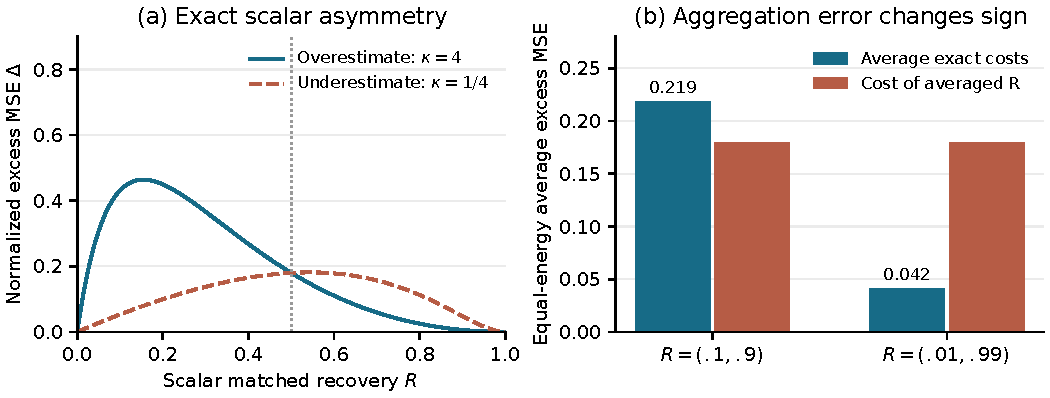
\includegraphics[width=.95\textwidth]{figures/scalar-cost.pdf}
\caption{Classical scalar cost and aggregation limits. Reciprocal mismatches cross at $R=.5$ under fixed effective noise. Equal-energy modes with the same mean $R=.5$ and $\kappa=4$ can give aggregation errors of either sign. These calculations do not identify a nonlinear network's effective prior.}\label{fig:cost}
\end{figure*}

\paragraph{Reference labels, not natural boundaries.} Historical protocols partition reference recovery at $.1$ and $.8$: A denotes high reference recovery, B intermediate and C low. These fixed labels permit the original test criteria to be audited. Their sensitivity has not been established, so we do not recommend them as deployment thresholds. With a fixed finite $\kappa$, the scalar excess vanishes as $R\to0$ or $1$, but the low-$R$ limit is not uniform over large mismatch factors. No reference label identifies the causal bottleneck of a trained decoder.

\paragraph{Band approximation.} A diagnostic sum
\begin{equation}\label{eq:crit}
C(Q)=\sum_b E_b\,\Delta\big(R_b,\kappa_b(Q)\big)
\end{equation}
substitutes measured band energies, reference recoveries and ratios of spectrum integrals. It is not the exact risk for a general operator. Its ranking accuracy and winner selection are distinct tests (\S\ref{sec:boundary}). Averaging $R$ and $\kappa$ before the nonlinear formula can either over- or under-estimate the true sum. For a fixed linear estimator the matrix expression in Appendix~\ref{app:linear} instead evaluates the specified covariance law directly.

\paragraph{No network mechanism follows.} A trained ASISR decoder is not a fixed Wiener estimator with known $\kappa$. Its measured $\Rnet$ is a truth-dependent outcome. Values near zero or one do not force a small readout-ablation loss: removing a component may improve a poorly recovered band or damage a perfectly recovered one. The loss ordering and scale-marginalisation tests in the main text therefore require empirical evidence independent of the scalar identity.

\section{Proof of Proposition~\ref{prop:mismatch}}\label{app:proof}
With $R=p/(p+q)$ the matched gain $R$ attains error $p(1-R)$. The gain
$g=\kappa p/(\kappa p+q)=\kappa R/(\kappa R+1-R)$ gives error
$(1-g)^2p+g^2q$. Using $q/p=(1-R)/R$ and $D=\kappa R+1-R$,
\[
\frac{(1-g)^2p+g^2q}{p}=\frac{(1-R)\big[(1-R)+\kappa^2R\big]}{D^2}.
\]
Subtracting $(1-R)$ and expanding $D^2$, the numerator becomes
$(1-R)\,R(1-R)(\kappa-1)^2$, which is Eq.~\eqref{eq:delta}.
For Cor.~\ref{cor:flip},
$\Delta(R,\kappa)/\Delta(R,1/\kappa)=\big((1-R)\kappa+R\big)^2/\big(1-R+\kappa R\big)^2$,
which exceeds 1 for $\kappa>1$ iff $(\kappa-1)(1-2R)>0$, i.e.\ iff $R<1/2$
(also checked numerically).

\section{Reproducibility}
Original sources, protocols and results retain their server directory
names in the collected evidence. The updated \texttt{SOURCES.md} maps each
claim to original or new output. New G1 and L2 runs invoke original frozen
evaluation code and preserve old results. The G1 protocol matches SHA256
prefix \texttt{548b26fe}; the full hash is recorded in \texttt{SOURCES.md}.
Independent L2 checking reconstructs pooled recoverability from saved
per-image signal/error arrays; G1 checking validates saved pooled numbers
and coverage, but per-image energy weights were not saved by its original
script. Exact machine-readable numerical checks accompany the evidence.

\section{Historical reference map}\label{app:map}
These prior simulations retain the original numerical values and fixed labels for source traceability. They do not use the natural-image E3 observation law: the latter has no injected noise and uses a different numerical variance. The labels are descriptive, with threshold sensitivity unverified.
\begin{table*}[t]\centering\small
\caption{Historical reference simulations: $\Rlin$ per band under the generic
$1/f^2$ prior, assumed spectrum and simulated observations; not a natural-image bound \src{OUT3/d8}.
Labels: A $\ge0.8$, B, C $<0.1$.}\label{tab:map}
\begin{adjustbox}{max width=\linewidth}\begin{tabular}{llccc}\toprule
Task & $\sigma_n$ & $b_1$ & $b_2$ & $b_3$\\\midrule
Single image $\times2$ & .002 / .01 & 1.00 / 1.00 & .92 / .90 & .09 / .08\\
Single image $\times4$ & .002 / .01 & .98 / .98 & .09 / .08 & .01 / .01\\
Single image $\times8$ & .002 / .01 & .79 / .77 & .01 / .01 & .01 / .01\\
Sparse 5\% & .002 & .70 & .09 & .03\\
Sparse 10\% & .002 & .81 & .20 & .07\\
Sparse 25\% & .002 & .92 & .47 & .20\\
Sparse 50\% & .002 & .98 & .76 & .46\\
Multi-frame $\times4$, $T{=}4$ & .002$\to$.02 & $\approx$1.0 & .73$\to$.51 & .12$\to$.03\\
Multi-frame $\times4$, $T{=}8$ & .002$\to$.02 & $\approx$1.0 & .83$\to$.62 & .27$\to$.08\\
Multi-frame $\times4$, $T{=}16$ & .002$\to$.02 & $\approx$1.0 & .90$\to$.73 & .41$\to$.15\\
\bottomrule\end{tabular}\end{adjustbox}
\end{table*}


\section{Matrix optimality and aggregation counterexamples}
Let $e_P=x-H_Py$. Since $\mathbb E[e_Py^\top]=0$, expanding
$x-Hy=e_P+(H_P-H)y$ cancels both cross terms. Multiplication by an arbitrary
fixed $W$ and taking traces gives the identity in Appendix~\ref{app:linear}.
Gaussianity is unnecessary for this second-moment calculation.

Even equal-energy modes with identical $\kappa=4$ demonstrate that band
plug-in costs have no uniform error direction. For $R=(.1,.9)$ the average
exact cost is .218639; for $R=(.01,.99)$ it is .041601. Both have average
$R=.5$, whose plug-in cost is .18: an underestimate in the first example
and an overestimate in the second. These examples do not use non-diagonal
sampling, so aggregation alone suffices. For fixed finite $\kappa>0$ the
cost vanishes as $R\to0$ or $1$, but the low-$R$ limit is not uniform in
$\kappa$: $R=.01$, $\kappa=100$ gives $\Delta=24.256863$.
The scalar identity was independently checked on a $101\times121$ grid
with maximum algebraic residual $7.2\times10^{-15}$ \src{CPU-10000}.


\section{Exploratory same-observation linear controls}\label{app:controls}
This development diagnostic separates a model's own uncertainty from
actual reconstruction error. It uses two already-seen images, DIV2K
0801/0802, one Fourier-feature seed and one paired noise draw; it is
neither a confirmatory comparison nor a new selection method.
A central native $128\times128$ crop is average-pooled to $64\times64$.
Two point-sampling frames use vertical stride four and horizontal phases
$(0,0)$, $(0,1)$ or $(0,2)$, each with 512 noisy RGB observations and
noise variance $\nu=10^{-4}$. Only horizontal phases change; this matched
point operator differs from E1's native integrated footprints.

All 24 linear predictions are fixed before truth-based scoring: two
images, three geometries, two scales $\sigma\in\{3,10\}$ and two kernels.
The RBF is $k_\sigma(u,v)=\exp[-2\pi^2\sigma^2\|u-v\|^2]$. The finite
Fourier kernel uses the original network's 256 frozen Gaussian frequencies,
with $\phi(u)=[\cos(2\pi Bu),\sin(2\pi Bu)]/\sqrt{256}$ and
$k(u,v)=\phi(u)^\top\phi(v)$. Both have unit diagonal, fixed mean $m=.5$
and ridge parameter $\nu$, solved in float64 by Cholesky. No bandwidth,
amplitude or regularisation search is performed. Saved nonlinear FF
outputs are compared without retraining. Fixed Fourier ridge is not the
MLP's full NTK or learned kernel \citep{tancik2020fourier}; its mean,
regularisation and optimisation also differ from those of the FF network.
The noise generator resets to the same seed for each geometry, giving
common random numbers across geometries.

Let $T=K_{to}(K_{oo}+\nu I)^{-1}$ for the $P$ scored target pixels.
Conditioning on a fixed clean RGB image, the exact raw-output risk over
fresh observation noise is
\begin{equation*}
\frac{\|T(X_o-m)-(X_t-m)\|_F^2}{3P}
+\frac{\nu\|T\|_F^2}{P}.
\end{equation*}
Truth is used only to score the bias term after the complete prediction
cohort is hash-frozen. For the saved noise draw, actual raw MSE further
includes its realised noise term and signed bias--noise cross term.
These identities do not apply after clamping, and are not observation-only
risk estimators. In contrast, $\operatorname{diag}(K_{tt}-TK_{ot})$ is
uncertainty under the candidate's own Gaussian prior. Different kernels
specify different target laws, so their own uncertainties are not a common
actual-risk comparison.

\begin{table}[t]
\centering\small
\begin{tabular}{lrrr}
\toprule
Estimator & $\sigma$ & 0801 & 0802 \\
\midrule
RBF & 3 & $+.763$ & $+.552$ \\
RBF & 10 & $+1.792$ & $+1.908$ \\
Fixed Fourier ridge & 3 & $+.480$ & $-1.125$ \\
Fixed Fourier ridge & 10 & $-.647$ & $-.664$ \\
Trained FF & 3 & $+.633$ & $+.443$ \\
Trained FF & 10 & $+.951$ & $+.919$ \\
\bottomrule
\end{tabular}
\caption{Development difference in clamped PSNR (dB), phase $(0,2)$ minus
$(0,1)$, on the identical shave-four region. All opposing signs are
retained; these two images and one seed do not establish a population
ordering or a nonlinear mechanism.}\label{tab:controls}
\end{table}

Table~\ref{tab:controls} has three opposing finite-Fourier comparisons.
At $\sigma=10$, phase $(0,2)$ has conditional expected \emph{raw} MSE
1.901/2.473 on 0801/0802, predominantly bias; clipping must not conceal
this failure. Within each fixed kernel/scale, model posterior variance
orders the three phases as $02<01<00$, while the conditional noise
propagation term orders them as $00<02<01$. Total conditional raw-risk
ordering agrees with model variance in only five of eight image/kernel/
scale combinations. Lower self-prior uncertainty therefore does not
certify lower fixed-image error.

On the discrete $56\times56$ target crop, phases $(0,1)$ and $(0,2)$
have exactly the same nearest-observation distance histogram. Continuous
periodic maximum gaps three/two alone cannot explain their different
errors, especially for these nonperiodic kernels and nonnested observation
sets. Covariance-parameter identifiability and reconstruction error are
different objects; this diagnostic supplies no general transfer theorem.
Joint correlations, prior mismatch and estimator behaviour require
separate analysis rather than a nearest-distance or rank-only mechanism.

All 24 controls finish with no numerical failure in 17.39 seconds of
shared CPU wall time (four threads, nice 10, 600-second absolute budget).
The complete prediction manifest precedes scoring; all saved outputs,
linear responses, residuals and failures are retained. Independent LU
recomputation of all 24 controls and primal/dual checking of all 12
Fourier controls agree with predictions within $2.51\times10^{-11}$.
These audits validate the calculations, not natural-image prior validity,
practical guidance or publication novelty \src{CTRL-20261008}.

As a common-law diagnostic, the same 12 distinct saved linear responses
are evaluated on 32 separate calibration crops, DIV2K 0001--0032, with
identical preprocessing, mean, noise variance and target region. Averaging
the preceding conditional-risk formula over these complete RGB images
defines a finite empirical evaluation law; no Gaussian or stationarity
assumption or population confidence interval is attached to it. All 384
image/operator risks and eight static recommendations are hash-frozen
before consulting the two development images. This is a retrospective
diagnostic designed after their earlier outcomes, not prospective evidence.
Calibration chooses RBF $\sigma=3$ within every geometry, and phase $(0,2)$
globally, agreeing with the conditional-risk optimum on both development
images. Across the overlapping eight choice groups per image, 15 of 16
recommendations match their oracle; the exception is Fourier ridge
$\sigma=3$ on 0801, with raw-risk regret .001037. Nevertheless, 15 of 132
pairwise comparisons have opposing signs. These dependent comparisons
do not establish a general transfer rate. The calibration recommendation
within each geometry coincides with the fixed RBF $\sigma=3$ baseline;
there is no image-adaptive gain. The complete CPU diagnostic takes 8.23
seconds without solving new systems or retraining \src{CAL-20261008}.

\section{Ambiguity, selection and unrestricted reconstruction}\label{app:ambiguity}
This elementary control illustrates classical robust decision principles,
not a new minimax theorem \citep{kitagawa2011inference}.
On eight periodic sites let $Q_k(i,j)=\tfrac14\cos[2\pi k(i-j)/8]$,
$D=Q_1-Q_3$, and $C_\pm=I\pm\theta D$, with known $0<\theta<1$,
unknown sign, zero mean and known noise variance $\nu>0$.
The priors are positive definite. Write $a=1+\nu$ and let $A_{01}$ and
$A_{02}$ select sites $(0,4,1,5)$ and $(0,4,2,6)$ respectively.
All risks below are total eight-coordinate squared error; divide by eight
for per-coordinate MSE.

For $A=A_{02}$, $ADA^\top=0$ and $\operatorname{tr}(AD^2A^\top)=2$.
Both worlds therefore have exactly the same observed Gaussian law,
$N(0,aI)$, and posterior means $m_\pm=A^\top y/a\pm\theta DA^\top y/a$.
Regret subtracts each world's own known-sign Bayes risk.
Their midpoint is an admissible mixture estimate. Posterior orthogonality
and the parallelogram identity give
\[
\frac{\operatorname{Reg}_+(g)+\operatorname{Reg}_-(g)}2
=\mathbb E\|g-A^\top y/a\|^2+\frac{2\theta^2}{a}.
\]
The midpoint attains both regrets equally, hence the unrestricted minimax
regret is $2\theta^2/a$ and total minimax risk is $8-4/a$.
Choosing only between $m_+$ and $m_-$ instead gives minimax regret
$4\theta^2/a$ when randomisation is allowed; fixed wrong selection costs
$8\theta^2/a$. Candidate-selection failure must not be promoted to the
same lower bound for all reconstruction methods.

The known-spectrum oracle favours $A_{02}$ by the positive risk gap
\[
\delta=R^*_{01}-R^*_{02}
=\frac{\theta^2(1+2\nu-\theta^2)}{a(a^2-\theta^2/2)}
<\frac{\theta^2}{a}.
\]
For $K$ independent calibration draws observed through the chosen
geometry, followed by a fresh evaluation draw, both designs pay
$4(K+1)$ measurements. Geometry 02 cannot learn the sign for any $K$.
Geometry 01 has distinct laws; calibration-only likelihood selection
has error at most $\tfrac12\exp[-K\theta^2/(4a^2)]$ and wrong-rule cost
$\Gamma=8a\theta^2(a^2-a+1/2)/(a^2-\theta^2/2)^2$.
It beats geometry 02's unrestricted worst-case total risk whenever
$\Gamma\exp[-K\theta^2/(4a^2)]/2<2\theta^2/a-\delta$.
This is a sufficient finite threshold, not a sharp transition or a new
general sampling law. Free full-resolution calibration or spectrum
labels would invalidate the information restriction. Prediction versus
covariance-learning design is already studied \citep{zimmerman2006optimal};
the present two-point illustration supplies no natural-image or INR
guarantee \src{SEP-20261008}.

\section{Finite-sample Gaussian confidence-set study}\label{app:confidence}
The completed frozen 8-point stationary Gaussian study contains 1920 cases under known zero mean, known noise and fixed trace-eight spectra. It uses independent same-law draws for selection and fresh-draw population risk for evaluation. All selections were hash-frozen before truth scoring. Of 1920 cases, 1887 confidence sets were nonempty, 33 empty and none reported numerical failure; the true spectrum lay in 1841 sets. Only 197 cases (10.26\% of the full cohort) yielded a recommendation certificate; no incorrect recommendation was observed among those 197. This does not mean zero error over the full cohort or safety on an adaptively reused single image. All 11322 valid LP endpoints and 384 diagnostic endpoints were independently recomputed. Strong empirical-Bayes performance and low certification coverage preclude a practical-advantage claim. The construction uses classical covariance estimation, partial identification and contrast-design ideas; it is not claimed as a new general sampling theorem. Protocols, null cases, raw outputs and full costs remain in the source ledger.

\end{document}
